\documentclass{article}
\usepackage[english]{babel}
\usepackage{blindtext}
\usepackage[hidelinks]{hyperref}
\usepackage[margin=0.5in]{geometry}
\usepackage{fancyhdr}
\usepackage{graphicx}
\usepackage{float}
\usepackage{booktabs}
\usepackage{titlesec}
\usepackage{tabularx}
\usepackage[shortlabels]{enumitem}

% \renewcommand\headrulewidth{0pt} % remove header rule
\fancyhf{}
\fancyhead[L]{\vspace{3mm}Session 2018--2022}
\fancyhead[R]{Software Cost and Effort Estimation System}
\fancyfoot[C]{\thepage}
\pagestyle{fancy}

\graphicspath{ {./} }

% Code to use \paragraph as \subsubsubsection ----

\makeatletter
\renewcommand\paragraph{\@startsection{paragraph}{4}{\z@}%
            {-2.5ex\@plus -1ex \@minus -.25ex}%
            {1.25ex \@plus .25ex}%
            {\normalfont\normalsize\bfseries}}
\makeatother
\setcounter{secnumdepth}{4} % how many sectioning levels to assign numbers to
\setcounter{tocdepth}{4}    % how many sectioning levels to show in ToC
% ---------------------------------------------------- 



\begin{document}


\pagenumbering{roman}

% Title Page
\graphicspath{ {./images/} }



\begin{center}
	\vspace{10mm}

	
\includegraphics[height=3.5cm, width=10cm]{logo} \\
	\vspace{10mm}

	\Huge{\textbf{Software Cost and Effort Estimation System}} \\
	\huge{A tool for software industries}
	\vspace{10mm}

	\Huge{\textbf{Final Year Project Documentation}} \\
	\vspace{20mm}

	\Large{\textbf{Submitted by}} \\
	\vspace{15mm}

	\Large{\textbf{Usman Ahmed \hspace{3cm} 70066997}}

	\vspace{1mm}

	\Large{\textbf{Faizan Ahmed \hspace{3cm} 70068241}}

	\vspace{10mm}

	\Large{\textbf{Project Supervisor}} \\
	\vspace{3mm}
	\Large{\textbf{Dr. Yasir Mehmood}}

	\vspace{15mm}


	\Large{\textbf{BACHELOR OF SCIENCE IN SOFTWARE ENGINEERING}} \\
	\vspace{10mm}
	\Large{\textbf{DEPARTMENT OF SOFTWARE ENGINEERING}} \\
	\vspace{3mm}
	\Large{\textbf{THE UNIVERSITY OF LAHORE}} \\






\end{center}


\pagebreak

% Signatures Page


\vspace{50mm}
\begin{center}

	
	\huge{\textbf{FINAL YEAR PROJECT PHASE-I DOCUMENTATION}} \\
	\vspace{10mm}

\end{center}

\vspace{20mm}

\begin{center}
	\huge{\textbf{STATEMENT OF SUBMISSION}} \\
	\vspace{10mm}

\end{center}


\vspace{20mm}


\begin{center}
	\Large{Submitted to the University of Lahore in partial fulfillment of the requirement for the award of degree of Bachelors of Science in Software Engineering (BSSE)} \\
	\vspace{10mm}

\end{center}
\vspace{10mm}
\Large

By
\vspace{10mm}

Usman Ahmed \hspace{5mm} (70066997) \hspace{5mm} \hrulefill

\vspace{5mm}

Faizan Ahmed \hspace{6mm} (70068241) \hspace{5mm} \hrulefill

\vspace{15mm}

\textbf{Project Advisor}
\hrulefill
\vspace{5mm}



\textbf{Dr Yasir Mahmood}
\vspace{5mm}


(Assistant Professor UOL)
\vspace{5mm}


Department of Software Engineering



\pagebreak


% Abstract, Dedication and Acknowledgements
\section*{Abstract}
\addcontentsline{toc}{section}{Abstract}
\blindtext
\newpage


\section*{Dedication}
\addcontentsline{toc}{section}{Dedication}
\blindtext
\newpage


\section*{Acknowledgements}
\addcontentsline{toc}{section}{Acknowledgements}
\blindtext
\newpage





% Table of contents page
\tableofcontents
\pagebreak

\listoffigures
\pagebreak



\pagenumbering{arabic}
% Chapter 1 Intorduction
%\section{Introduction}

\vspace{20mm}

\Huge{\textbf{Introduction to Problem}}

\vspace{20mm}


\begin{abstract}
	In this chapter, we will be introducing the problem and the requirements that will be used to solve it. The purpose and main objectives that are at the core of the project will be explained in a concise manner. Along with those details we will also discuss the already existing solutions to the current problem and how these existing solutions are no longer a viable choice for consumers. We shall also discuss how our solution fixes the issues that were found in the existing solutions and how our solution/product will be a superior and generally better. After these details an executive summary will summarize all of the above discussions into a concise manner.
\end{abstract}

\vspace{20mm}






\large{\textbf{Outline}}

\begin{center}
	\begin{itemize}
		\item Introduction
		\item Purpose
		\item Objectives
		\item Existing Solutions
		\item Proposed Solution
		\item Novelty
		\item Executive Summary
	\end{itemize}
\end{center}
\pagebreak








\subsection{Introduction}
The software industry is a multi billion dollar industry, infact it is projected to be around 1 trillion USD in 2023. This is due to the fact that software development is complex and requires a lot of resources. And just like any complex engineering project, much of these resources, time and effort goes into planning the development of the project. Successfull software developers and companies realize the importance of a well organized and well planned software development process. Without one, the project will more than likely fail to be completed. {\it{"Without requirements or design , programming is the art of adding bugs to an empty text file"}}, a humourous quote from Louis Srygley, well summarizes the need for  a well planned and estimated software development process.
\vspace{2mm}

After all the planning and design phases, team leads and managers have to come up with a time and resource estimate for the project. This is a crucial phase and a lot can go wrong here. According to a survey over 60\% of software projects fail to complete in the estimated time and budget. 












\subsection{Purpose}
The main pupose of our product is to improve the accuracy of estimate predictions. This will be done using state-of-the-art machine learning algorithms that are trained on previous software development projects. The classifier will also improve significantly with the passage of time, since we will be recording statistics of all the projects that will be entered in the product. 

 The secondary puspose is to provide a platform where developers and managers can collaborate and share their options on the project's development and create estimates manually. Our product will basically give it's users the option to choose between different estimation techniques but the recommended techinique will still be the machine learnign classifier.












\subsection{Objective}
Following are the most important objectives of the project.
\begin{itemize}
	\item Improve the accuracy of software cost and effort estimation techniques.
	\item Get upto 50\% of software development organizations to swtich to automated software cost and effort estimation techniques.
	\item Get managers to switch to our product by automating their current estimation workflows and then  integrating our specialized techiniques with their existing workflows.
	\item Making our product compatible with most of today's tredning programming languages and their popular frameworks.
	\item Making our product relevant among the software development organizations and get 20 large software development organizations and/or 50 medium scale organizations to switch to our product by the end of 2023. And to integrate our product with their existing management routines.
\end{itemize}













\subsection{Existing Solutions}
There are a few existing solutions in this problem space. Some of them are now not maintained and are deprecated. Following is a list of similar projects
\begin{itemize}
	\item {\bf{SEER For Software}}\newline
	SEER is a general purpose estimation tool that also has a product for software projects' estimation. It accepts input in form of SLOC (Source lines of code), function points, use cases and some more less popular options. After processing these inputs using proprietary models, the output of the program is as follows: Project time duration, development hours and accuracy of estimations.

	\item {\bf{TruePlanning \small{\textregistered}}}\newline
	This product is calculates its estimates using the PRICE model. Developed in 1975, TruePlanning is also a general purpose estimation system.
	
\end{itemize}













\subsection{Disadvantages}
Following are some serious shortcomings or disadvantages with the currently existing solutions
\begin{itemize}
	\item Outdated models that cannot adapt to today's rapidly changing and extremely diverse development languages and frameworks.
	\item No platform to enable communication between management and developers to discuss and agree to a better estimate
	\item Older and less commonly used input formats like SLOC and function points
	\item Outdated subscription methods. All of these prgorams implement a {\it{One Time Payment}} method. The disadvantage here is that the one time payment is a huge sum of money and may throw off a potential customer's interest in the product.
\end{itemize}









\subsection{Purposd Solution}
\blindtext[2]







\subsection{Novelty}
\blindtext[1]








\subsection{Executive Summary}
\blindtext[2]



% Chapter 2 Software Requirements Specification
%\section{Software Requirements Specification}

\vspace{20mm}



\begin{abstract}
	In this chapter, We will discuss our
    functional requirements and non-functional
    requirements that will be used later on. There are two types of 
    requirements i.e Functional Requirement and Non-Functional Requirements.
    functional requirements define what the system does or must not do, non-functional
    requirements specify how the system should do it. Non-functional requirements do not
    affect the basic functionality of the system (hence the name, non-functional requirements).
    
\end{abstract}

\vspace{20mm}

\large{\textbf{Outline}}

\begin{center}
    \begin{itemize}
        \item Introduction
              \begin{itemize}
                  \item Purpose
                  \item Scope
              \end{itemize}
        \item Overall Description
        \item User Characteristics
        \item Specific Requirements
              \begin{itemize}
                  \item Functional Requirements
                  \item Non-Functional Requirements
              \end{itemize}
    \end{itemize}
\end{center}
\pagebreak


\subsection{Introduction}

    \subsubsection{Purpose}
    Here, is the purpose of our project is that the Cost Estimation is major component
    of planning a large scale software project.A wrong estimate of the project’s effort
    can lead to disastrous outcomes.Project managers can under estimate as well as 
    overestimate a project’s effort, so it is crucial to correctly estimate the 
    complexity of our project in order to deliver the product on time, provide a 
    much better developer experience and most importantly, don’t go over budget.


    \subsubsection{Scope}
    The major Scope of our Project is to estimate actual cost of the project and helpful to managers of the software industry are likely easy to calculate the budget of the developing software, and also ease to assigned the developer to the particular developing software.
    
    \subsubsection{Definition acronym \& abbrevation}
    The following acronym are used in our documents
    \begin{center}
        \begin{itemize}
            \item {\bfseries MERN:} MongoDB ExpressJS ReactJS NodeJS
            \item {\bfseries REST:} Restfull
            \item {\bfseries API:} Application Programming Interface
            \item {\bfseries DB:} Database
            \item {\bfseries SRS:} Software Requirements Specification
            \item {\bfseries UCP:} Use Case Point
            \item {\bfseries SPA:} Single Page Application
            \item {\bfseries CBR:} Content Base Reasoning
            \item {\bfseries FRs:} Functional Requirements
            \item {\bfseries NFRs:} Non-Functional Requirements
            \end{itemize}
    \end{center}
    
% continue from their
\subsection{Overall Description}
\subsubsection{Product Perspective}
Our Final Year Project is SPA(Single Page Application). To reduce the difficulties for those managers who feels 
difficulties to estimate the actual effort/cost of the upcoming project. Managers can also some other modules except
the Estimation i.e {\bfseries View/Update project} and {\bfseries Add/Remove Developers} in a project. Other than manager, there is a developer module in which developer 
can View and inform estimation of the project. Manager also have option to use our all methods for estimation as well as choose only one or two for calculating the actual estimate of the project.

    
\subsection{User Characteristics}
\blindtext[2]

\subsection{Specific Requirements}
\blindtext[2]

\subsubsection{Functional Requirements}
\newcommand{\splitcell}[2][c]{%
  \begin{tabular}[#1]{@{}c@{}}#2\end{tabular}}
\subsubsection{FR-01: Register}
\begin{center}
  \begin{tabularx}{\textwidth}{|l|X|}
      \hline
      \textbf{ID} & FR-01 \\
      \hline
      \textbf{Name} & Register \\
      \hline
      \textbf{Description} & Register a new user \\
      \hline
      \textbf{Input} & username, password, password\_confirmation, email \\
      \hline
      \textbf{Output} & A new user is created in the database \\
      \hline
      \textbf{Requirements} & Valid username, valid email, password that contains at least 8 characters, password\_confirmation that matches the password \\
      \hline
  \end{tabularx}
\end{center}

\subsubsection{FR-02: Login}
\begin{center}
  \begin{tabularx}{\textwidth}{|l|X|}
      \hline
      \textbf{ID} & FR-02 \\
      \hline
      \textbf{Name} & Login \\
      \hline
      \textbf{Description} & Login to the application \\
      \hline
      \textbf{Input} & username or email, password \\
      \hline
      \textbf{Output} & User is logged in, a JWT token is issued \\
      \hline
      \textbf{Requirements} & Valid username or email, matching password \\
      \hline
  \end{tabularx}
\end{center}

\subsubsection{FR-03: OAuth}
\begin{center}
  \begin{tabularx}{\textwidth}{|l|X|}
      \hline
      \textbf{ID} & FR-03 \\
      \hline
      \textbf{Name} & OAuth \\
      \hline
      \textbf{Description} & Login to the application using OAuth \\
      \hline
      \textbf{Input} & OAuth token \\
      \hline
      \textbf{Output} & User is logged in, a JWT token is issued \\
      \hline
      \textbf{Requirements} & Valid OAuth token \\
      \hline
  \end{tabularx}
\end{center}

\subsubsection{FR-04: Forget Password}
\begin{center}
  \begin{tabularx}{\textwidth}{|l|X|}
      \hline
      \textbf{ID} & FR-04 \\
      \hline
      \textbf{Name} & Forgot password \\
      \hline
      \textbf{Description} & Send an email to the user with a link to reset their password \\
      \hline
      \textbf{Input} & email \\
      \hline
      \textbf{Output} & An email is sent to the user with a link to reset their password \\
      \hline
      \textbf{Requirements} & Valid email \\
      \hline
  \end{tabularx}
\end{center}
\newpage

\subsubsection{FR-05: Reset Password}
\begin{center}
  \begin{tabularx}{\textwidth}{|l|X|}
      \hline
      \textbf{ID} & FR-05 \\
      \hline
      \textbf{Name} & Reset password \\
      \hline
      \textbf{Description} & Reset the user's password \\
      \hline
      \textbf{Input} & token, password, password\_confirmation \\
      \hline
      \textbf{Output} & The user's password is reset \\
      \hline
      \textbf{Requirements} & Valid token, valid password, password\_confirmation that matches the password \\
      \hline
  \end{tabularx}
\end{center}


\subsubsection{FR-06: Confirm Account}
\begin{center}
  \begin{tabularx}{\textwidth}{|l|X|}
      \hline
      \textbf{ID} & FR-06 \\
      \hline
      \textbf{Name} & Confirm account \\
      \hline
      \textbf{Description} & Confirm the user's account \\
      \hline
      \textbf{Input} & token \\
      \hline
      \textbf{Output} & The user's account is confirmed \\
      \hline
      \textbf{Requirements} & Valid token \\
      \hline
  \end{tabularx}
\end{center}

\subsubsection{FR-07: Delete Account}
\begin{center}
  \begin{tabularx}{\textwidth}{|l|X|}
      \hline
      \textbf{ID} & FR-07 \\
      \hline
      \textbf{Name} & Delete account \\
      \hline
      \textbf{Description} & Delete the user's account \\
      \hline
      \textbf{Input} & token \\
      \hline
      \textbf{Output} & The user's account is deleted \\
      \hline
      \textbf{Requirements} & Valid token \\
      \hline
  \end{tabularx}
\end{center}

\subsubsection{FR-08: Create Initial Account}
\begin{center}
  \begin{tabularx}{\textwidth}{|l|X|}
      \hline
      \textbf{ID} & FR-08 \\
      \hline
      \textbf{Name} & Create initial account \\
      \hline
      \textbf{Description} & Create the initial account \\
      \hline
      \textbf{Input} & role \\
      \hline
      \textbf{Output} & A user's information is complete \\
      \hline
      \textbf{Requirements} & A role, either developer or manager \\
      \hline
  \end{tabularx}
\end{center}

\subsubsection{FR-09: Create Initial Account usmanError}
\begin{center}
  \begin{tabularx}{\textwidth}{|l|X|}
      \hline
      \textbf{ID} & FR-09 \\
      \hline
      \textbf{Name} & Create initial account \\
      \hline
      \textbf{Description} & Create the initial account \\
      \hline
      \textbf{Input} & username, password, email \\
      \hline
      \textbf{Output} & The initial account is created \\
      \hline
      \textbf{Requirements} & Valid username, valid email, password that contains at least 8 characters \\
      \hline
  \end{tabularx}
\end{center}

\subsubsection{FR-10: Edit Account Info.}
\begin{center}
  \begin{tabularx}{\textwidth}{|l|X|}
      \hline
      \textbf{ID} & FR-10 \\
      \hline
      \textbf{Name} & Edit account info \\
      \hline
      \textbf{Description} & Edit the user's account info \\
      \hline
      \textbf{Input} & token, username, email \\
      \hline
      \textbf{Output} & The user's account info is updated \\
      \hline
      \textbf{Requirements} & Valid token, valid username, valid email \\
      \hline
  \end{tabularx}
\end{center}

\subsubsection{FR-11: Edit Interface Preference}
\begin{center}
  \begin{tabularx}{\textwidth}{|l|X|}
      \hline
      \textbf{ID} & FR-11 \\
      \hline
      \textbf{Name} & Edit interface preferences \\
      \hline
      \textbf{Description} & Edit the user's interface preferences \\
      \hline
      \textbf{Input} & token, theme, language \\
      \hline
      \textbf{Output} & The user's interface preferences are updated \\
      \hline
      \textbf{Requirements} & Valid token, valid theme, valid language \\
      \hline
  \end{tabularx}
\end{center}

\subsubsection{FR-12: Create Project}
\begin{center}
  \begin{tabularx}{\textwidth}{|l|X|}
      \hline
      \textbf{ID} & FR-12 \\
      \hline
      \textbf{Name} & Create Project \\
      \hline
      \textbf{Description} & The manager creates a fresh project \\
      \hline
      \textbf{Input} & use cases (file/forms), add developers(optional), project name, technology \\
      \hline
      \textbf{Output} & A new project is created in the database with the ID of its manager \\
      \hline
      \textbf{Requirements} & Use cases, name, technology name \\
      \hline
  \end{tabularx}
\end{center}

\subsubsection{FR-13: Edit Project}
\begin{center}
  \begin{tabularx}{\textwidth}{|l|X|}
      \hline
      \textbf{ID} & FR-13 \\
      \hline
      \textbf{Name} & Edit Project \\
      \hline
      \textbf{Description} & The manager edits an existing project \\
      \hline
      \textbf{Input} & use cases (file/forms), project name, technology, (all optional), project ID(needed) \\
      \hline
      \textbf{Output} & The referred project is  \\
      \hline
      \textbf{Requirements} & Use cases, name, technology name, manager logged in, project exists \\
      \hline
  \end{tabularx}
\end{center}

\subsubsection{FR-14: Delete Project}
\begin{center}
  \begin{tabularx}{\textwidth}{|l|X|}
      \hline
      \textbf{ID} & FR-14 \\
      \hline
      \textbf{Name} & Delete Project \\
      \hline
      \textbf{Description} & The manager removes an existing project from database \\
      \hline
      \textbf{Input} & Manager clicks on delete project and clicks Yes \\
      \hline
      \textbf{Output} & The referred project is removed from database \\
      \hline
      \textbf{Requirements} & Project ID, manager logged in \\
      \hline
  \end{tabularx}
\end{center}

\subsubsection{FR-15: Add Developer}
\begin{center}
  \begin{tabularx}{\textwidth}{|l|X|}
      \hline
      \textbf{ID} & FR-15 \\
      \hline
      \textbf{Name} & Add Developer \\
      \hline
      \textbf{Description} & The manager assigns a developer to the project \\
      \hline
      \textbf{Input} & Manager clicks on add new developer and types developer's username \\
      \hline
      \textbf{Output} & A new developer is added to projects developer's list \\
      \hline
      \textbf{Requirements} & Project ID, manager logged in, developer username \\
      \hline
  \end{tabularx}
\end{center}

\subsubsection{FR-16: Remove Developer}
\begin{center}
  \begin{tabularx}{\textwidth}{|l|X|}
      \hline
      \textbf{ID} & FR-16 \\
      \hline
      \textbf{Name} & Remove Developer \\
      \hline
      \textbf{Description} & The manager removes a developer from the project \\
      \hline
      \textbf{Input} & Manager goes into developers list and clicks remove button and then clicks Yes \\
      \hline
      \textbf{Output} & The developer is removed from the project's developers list \\
      \hline
      \textbf{Requirements} & Project ID, manager logged in, developer username \\
      \hline
  \end{tabularx}
\end{center}

\subsubsection{FR-17: Edit Developer Permission}
\begin{center}
  \begin{tabularx}{\textwidth}{|l|X|}
      \hline
      \textbf{ID} & FR-17 \\
      \hline
      \textbf{Name} & Edit Developer Permissions \\
      \hline
      \textbf{Description} & Manager changes a developer's access level to the project \\
      \hline
      \textbf{Input} & Manager goes tp developers list and clicks on change role on a developer. They then choose either View or Edit \\
      \hline
      \textbf{Output} & Project permissions are edited \\
      \hline
      \textbf{Requirements} & Project ID, Developer ID, Permission type, manager logged in \\
      \hline
  \end{tabularx}
\end{center}

\subsubsection{FR-18: Calculate UCP}
\begin{center}
  \begin{tabularx}{\textwidth}{|l|X|}
      \hline
      \textbf{ID} & FR-18 \\
      \hline
      \textbf{Name} & Calculate UCP \\
      \hline
      \textbf{Description} & Get UCP estimation of project using use cases \\
      \hline
      \textbf{Input} & Use Cases, environmental factors, technical factors \\
      \hline
      \textbf{Output} & An integer representing the UCP estimation in man hours \\
      \hline
      \textbf{Requirements} & manager logged in, use at least 2 cases are entered \\
      \hline
  \end{tabularx}
\end{center}

\subsubsection{FR-19: Get Machine Learning Estimate}
\begin{center}
  \begin{tabularx}{\textwidth}{|l|X|}
      \hline
      \textbf{ID} & FR-19 \\
      \hline
      \textbf{Name} & Get Machine Learning Estimate \\
      \hline
      \textbf{Description} & Calculate estimate using machine learning model \\
      \hline
      \textbf{Input} & Use Cases, environmental factors, technical factors \\
      \hline
      \textbf{Output} & An integer representing the machine learning estimation in man hours \\
      \hline
      \textbf{Requirements} & manager logged in, use at least 2 cases are entered \\
      \hline
  \end{tabularx}
\end{center}

\subsubsection{FR-20: Start Manual Estimation Round}
\begin{center}
  \begin{tabularx}{\textwidth}{|l|X|}
      \hline
      \textbf{ID} & FR-20 \\
      \hline
      \textbf{Name} & Start Manual Estimation Round \\
      \hline
      \textbf{Description} & Create an empty round in current project \\
      \hline
      \textbf{Input} & Manager clicks on start manual estimation \\
      \hline
      \textbf{Output} & Empty round is created in database for current project \\
      \hline
      \textbf{Requirements} & Manager logged in, project exists, project has at least two use case, at least one developer assigned to project \\
      \hline
  \end{tabularx}
\end{center}

\subsubsection{FR-21: End Round}
\begin{center}
  \begin{tabularx}{\textwidth}{|l|X|}
      \hline
      \textbf{ID} & FR-21 \\
      \hline
      \textbf{Name} & End Round \\
      \hline
      \textbf{Description} & End current round, locking in all estimates given so far \\
      \hline
      \textbf{Input} & Manager clicks end round \\
      \hline
      \textbf{Output} & Round length is increased by one and all estimates are locked in \\
      \hline
      \textbf{Requirements} & Round exists, manager logged in, at least one estimate is made \\
      \hline
  \end{tabularx}
\end{center}

\subsubsection{FR-22: Clear Round}
\begin{center}
  \begin{tabularx}{\textwidth}{|l|X|}
      \hline
      \textbf{ID} & FR-22 \\
      \hline
      \textbf{Name} & Clear Round \\
      \hline
      \textbf{Description} & Clear current round's estimates \\
      \hline
      \textbf{Input} & Manager clicks on clear round \\
      \hline
      \textbf{Output} & All of estimates made for this round are deleted \\
      \hline
      \textbf{Requirements} & Round exists, manager logged in, at least one estimate is made \\
      \hline
  \end{tabularx}
\end{center}

\subsubsection{FR-23: Calculate Round Average}
\begin{center}
  \begin{tabularx}{\textwidth}{|l|X|}
      \hline
      \textbf{ID} & FR-23 \\
      \hline
      \textbf{Name} & Calculate Round Average \\
      \hline
      \textbf{Description} & Process all given estimates and calculate average \\
      \hline
      \textbf{Input} & A round is finished \\
      \hline
      \textbf{Output} & Average is calculated and stored in database for current round \\
      \hline
      \textbf{Requirements} & Round exists, manager logged in, at least one estimate is made \\
      \hline
  \end{tabularx}
\end{center}

\subsubsection{FR-24: Finalize Manual Estimation}
\begin{center}
  \begin{tabularx}{\textwidth}{|l|X|}
      \hline
      \textbf{ID} & FR-24 \\
      \hline
      \textbf{Name} & Finalize Manual Estimation \\
      \hline
      \textbf{Description} & Multiple rounds are finished and the team has agreed on a final estimate \\
      \hline
      \textbf{Input} & Manager clicks on finalize button \\
      \hline
      \textbf{Output} & Manual estimation is calculated and stored in database for current round \\
      \hline
      \textbf{Requirements} & Al least one round finished, manager logged in \\
      \hline
  \end{tabularx}
\end{center}

\subsubsection{FR-25: AllEstimate Bar Chart}
\begin{center}
  \begin{tabularx}{\textwidth}{|l|X|}
      \hline
      \textbf{ID} & FR-25 \\
      \hline
      \textbf{Name} & All Estimate Bar Chart \\
      \hline
      \textbf{Description} & Generate a bar chart comparing all types of estimates \\
      \hline
      \textbf{Input} & UCP estimate, manual estimate, ML estimate \\
      \hline
      \textbf{Output} & A bar chart is generated \\
      \hline
      \textbf{Requirements} & At least one type of estimate calculated \\
      \hline
  \end{tabularx}
\end{center}

\subsubsection{FR-26: All Manual Estimate Rounds' Line Chart}
\begin{center}
  \begin{tabularx}{\textwidth}{|l|X|}
      \hline
      \textbf{ID} & FR-26 \\
      \hline
      \textbf{Name} & All Manual Estimate Rounds' Line Chart \\
      \hline
      \textbf{Description} & A line chart of all rounds' estimates generated overtime \\
      \hline
      \textbf{Input} & All rounds' averages \\
      \hline
      \textbf{Output} & A line chart is generated \\
      \hline
      \textbf{Requirements} & At least one round has been finished \\
      \hline
  \end{tabularx}
\end{center}

\subsubsection{FR-27: All Manual Estimate Rounds' Bar Chart usman ERROR}
\begin{center}
  \begin{tabularx}{\textwidth}{|l|X|}
      \hline
      \textbf{ID} & FR-27 \\
      \hline
      \textbf{Name} & All Manual Estimate Rounds' Bar Chart \\
      \hline
      \textbf{Description} & A bar chart with showing the progressing of manual estimation rounds while highlighting each developer's estimate \\
      \hline
      \textbf{Input} & round estimates , developers' estimates \\
      \hline
      \textbf{Output} & A bar chart is generated \\
      \hline
      \textbf{Requirements} & At least one round has been finished \\
      \hline
  \end{tabularx}
\end{center}

\subsubsection{FR-28: All Machine Learning Estimates Line Chart}
\begin{center}
  \begin{tabularx}{\textwidth}{|l|X|}
      \hline
      \textbf{ID} & FR-28 \\
      \hline
      \textbf{Name} & All Machine Learning Estimates Line Chart \\
      \hline
      \textbf{Description} & Generate a line chart of all machine learning estimates so far \\
      \hline
      \textbf{Input} & Machine learning estimates \\
      \hline
      \textbf{Output} & A line chart is generated \\
      \hline
      \textbf{Requirements} & At least one ML estimate calculated \\
      \hline
  \end{tabularx}
\end{center}

\subsubsection{FR-29: Pie Chart of Use Cases Weight}
\begin{center}
  \begin{tabularx}{\textwidth}{|l|X|}
      \hline
      \textbf{ID} & FR-29 \\
      \hline
      \textbf{Name} & Pie Chart of Use Cases Weight \\
      \hline
      \textbf{Description} & A pie chart showcasing the most important use cases \\
      \hline
      \textbf{Input} & Use cases \\
      \hline
      \textbf{Output} & A pie chart is generated \\
      \hline
      \textbf{Requirements} & At least two use cases are entered \\
      \hline
  \end{tabularx}
\end{center}

\subsubsection{FR-30: Template of FR}
\begin{center}
  \begin{tabularx}{\textwidth}{|l|X|}
      \hline
      \textbf{ID} & FR-30 \\
      \hline
      \textbf{Name} &  \\
      \hline
      \textbf{Description} &  \\
      \hline
      \textbf{Input} &  \\
      \hline
      \textbf{Output} &  \\
      \hline
      \textbf{Requirements} &  \\
      \hline
  \end{tabularx}
\end{center}

\subsection{Non Functional Requirements}


\newpage

% \begin{center}
%     \begin{table}[H]
%         \centering
%         \begin{tabular}{@{}|l|l|l|l|@{}}
%             \hline
%             ID                           & \multicolumn{3}{l|}{FR-01}                                                                \\ \midrule
%             Name                         & \multicolumn{3}{l|}{Admin Sign-Up}                                                        \\ \midrule
%             Description                  & Input                              & Output                   & Basic Workflow            \\ \midrule
%             Admin register their account & \begin{tabular}[c]{@{}l@{}}User name and password must be \\ greater than eight letters\\ Details of user\end{tabular}          & Creation of User account & \begin{tabular}[c]{@{}l@{}}Enter user details and  added\\ into the database records\end{tabular} \\ \bottomrule
%         \end{tabular}
%         \caption{Functional Requirement 01: Admin Sign-Up}
%         \label{table:FR01}
%     \end{table}
% \end{center}




% Chapter 3 Use Case Analysis
%\setcounter{figure}{0}
\subsubsection{UC-01: Register}
    \begin{figure}[H]
    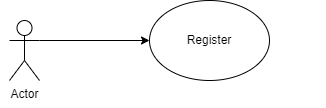
\includegraphics[height=5cm, width=0.8\textwidth]{./diagrams/Use Case/u1.png}
    \centering 
    \caption{Use Case Diagram for Registeration}
    \label{figure1}
    \end{figure}
    
    \begin{center}
        \begin{tabularx}{\textwidth}{|l|X|}
            \hline
            \textbf{ID} & UC-01 \\
            \hline
            \textbf{Name} & Register \\
            \hline
            \textbf{Description} & User can register their to keep their role in that software \\
            \hline
            \textbf{Actors} & New User \\
            \hline
            \textbf{Triggers} & Just Connect to in the internet and a email address \\
            \hline
            \textbf{Pre Conditions} & None \\
            \hline
            \textbf{Post Conditions} & Account Created Succesfully \\
            \hline
            \textbf{Main Course} & 1. Enter their Details \\2.Create their accound according to their given details \\
            \hline
            \textbf{Alternative Course} & Error due to invalid details \\
            \hline
            
        \end{tabularx}
    \end{center}
    \newpage
    

    \subsubsection{UC-02: Login}
    \begin{figure}[H]
        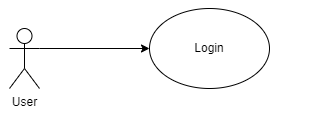
\includegraphics[height=5cm, width=0.8\textwidth]{./diagrams/Use Case/u2.png}
        \centering 
        \caption{Use Case Diagram for Login}
        \label{Usecase1}
        \end{figure}
        
    
    \begin{center}
        \begin{tabularx}{\textwidth}{|l|X|}
            \hline
            \textbf{ID} & UC-02 \\
            \hline
            \textbf{Name} & Login \\
            \hline
            \textbf{Description} & Login to the system to view/change in their account \\
            \hline
            \textbf{Actors} & New User \\
            \hline
            \textbf{Triggers} & just confirm with email which they provided in sign up \\
            \hline
            \textbf{Pre Conditions} & they must have a account \\
            \hline
            \textbf{Post Conditions} & they succesfully see the dashboard and more settings and features \\
            \hline
            \textbf{Main Course} & User can enter/use their email and its valid password \\
            \hline
            \textbf{Alternative Course} & Error due to invalid details \\
            \hline
            
        \end{tabularx}
    \end{center}
    \newpage
    

    \subsubsection{UC-03: OAuth}
    \begin{figure}[H]
        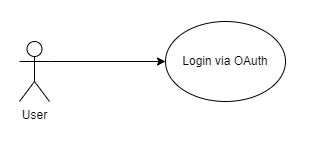
\includegraphics[height=5cm, width=0.8\textwidth]{./diagrams/Use Case/u3.png}
        \centering 
        \caption{Use Case Diagram for Login via OAuth}
        \label{Usecase1}
        \end{figure}
        
    \begin{center}
        \begin{tabularx}{\textwidth}{|l|X|}
            \hline
            \textbf{ID} & UC-03 \\
            \hline
            \textbf{Name} & OAuth \\
            \hline
            \textbf{Description} & User can ouath their details with third party like Gmail , LinkdIn and Github \\
            \hline
            \textbf{Actors} & New User \\
            \hline
            \textbf{Triggers} & Just have a third party account  \\
            \hline
            \textbf{Pre Conditions} & None \\
            \hline
            \textbf{Post Conditions} & Account has created by confiramtion through email  \\
            \hline
            \textbf{Main Course} & User can create their account on system by sending a email confirmation token. \\
            \hline
            \textbf{Alternative Course} & Error will show if you cant verify your third party account \\
            \hline
            
        \end{tabularx}
    \end{center}
    \newpage
    

    \subsubsection{UC-04: Forget Password}
    \begin{figure}[H]
        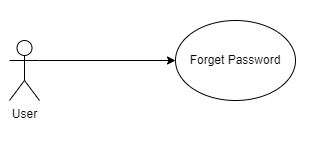
\includegraphics[height=5cm, width=0.8\textwidth]{./diagrams/Use Case/u4.png}
        \centering 
        \caption{Use Case Diagram for Forget Password}
        \label{fig: Usecase1}
        \end{figure}
        
    \begin{center}
        \begin{tabularx}{\textwidth}{|l|X|}
            \hline
            \textbf{ID} & UC-04 \\
            \hline
            \textbf{Name} & Forget Password \\
            \hline
            \textbf{Description} & Send the email to the user with a link to reset their password \\
            \hline
            \textbf{Actors} & Account Holder \\
            \hline
           \textbf{Triggers} & Send a link to the provided email for verfication purposes \\
            \hline
            \textbf{Pre Conditions} & Valid Email \\
            \hline
            \textbf{Post Conditions} & New password has been changed \\
            \hline
            \textbf{Main Course} & User can change their password by sending link to their email and setting the new password with the password requirements \\
            \hline
            \textbf{Alternative Course} & Error will be show due to invalid details \\
            \hline
            
        \end{tabularx}
    \end{center}
    \newpage
    

    \subsubsection{UC-05: Reset Password}
    \begin{figure}[H]
        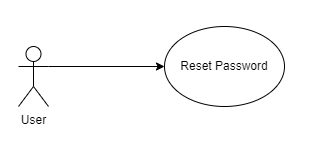
\includegraphics[height=5cm, width=0.8\textwidth]{./diagrams/Use Case/u5.png}
        \centering 
        \caption{Use Case Diagram for Reset Password}
        \label{fig:Usecase1}
        \end{figure}
        
    \begin{center}
        \begin{tabularx}{\textwidth}{|l|X|}
            \hline
            \textbf{ID} & UC-05 \\
            \hline
            \textbf{Name} & Reset Password \\
            \hline
            \textbf{Description} & User can reset/change your password by entering you current password \\
            \hline
            \textbf{Actors} & Account Holder \\
            \hline
            \textbf{Triggers} & You can reset/change the password before entering current password and the activity will be send on provided email\\
            \hline
            \textbf{Pre Conditions} & User have a account \\
            \hline
            \textbf{Post Conditions} & Password has been reset/change \\
            \hline
            \textbf{Main Course} & User can reset their password by entering their current password and password will set to new updated password \\
            \hline
            \textbf{Alternative Course} & Error will be show due to invalid details \\
            \hline
            
        \end{tabularx}
    \end{center}
    \newpage
    

    \subsubsection{UC-06: Confirm Account}
    \begin{figure}[H]
        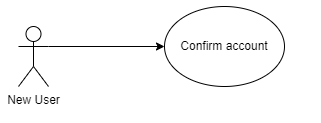
\includegraphics[height=5cm, width=0.8\textwidth]{./diagrams/Use Case/u6.png}
        \centering 
        \caption{Use Case Diagram for Confirm Account}
        \label{fig:Usecase1}
        \end{figure}
        
    \begin{center}
        \begin{tabularx}{\textwidth}{|l|X|}
            \hline
            \textbf{ID} & UC-06 \\
            \hline
            \textbf{Name} & Confirm Account \\
            \hline
            \textbf{Description} & User can confirm their account by a valid email address \\
            \hline
            \textbf{Actors} & New User \\
            \hline
            \textbf{Triggers} & By send the valid link to user's provided email \\
            \hline
            \textbf{Pre Conditions} & Fill the signup form \\
            \hline
            \textbf{Post Conditions} & account verified \\
            \hline
            \textbf{Main Course} & Account has been created though 3rd Party validation \\
            \hline
            \textbf{Alternative Course} & Error by unvalid email provided \\
            \hline
            
        \end{tabularx}
    \end{center}
    \newpage
    

    \subsubsection{UC-07: Delete Account}
    \begin{figure}[H]
        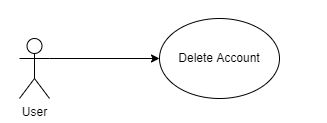
\includegraphics[height=5cm, width=0.8\textwidth]{./diagrams/Use Case/u7.png}
        \centering 
        \caption{Use Case Diagram for Delete Account}
        \label{fig:Usecase1}
        \end{figure}
        
    \begin{center}
        \begin{tabularx}{\textwidth}{|l|X|}
            \hline
            \textbf{ID} & UC-07 \\
            \hline
            \textbf{Name} & Delete Account \\
            \hline
            \textbf{Description} & User can delete the account if he/she can \\
            \hline
            \textbf{Actors} & Already User \\
            \hline
            \textbf{Triggers} & remove the user\_id from database by click on reset button \\
            \hline
            \textbf{Pre Conditions} & Already user database was be present in database \\
            \hline
            \textbf{Post Conditions} & No user of that user\_id will not be in database \\
            \hline
            \textbf{Main Course} & Account has been removed from database by the confirmation of user \\
            \hline
            \textbf{Alternative Course} & Error will be appeared by database \\
            \hline
            
        \end{tabularx}
    \end{center}
    \newpage
    

    \subsubsection{UC-08: Edit Account Info}
    \begin{figure}[H]
        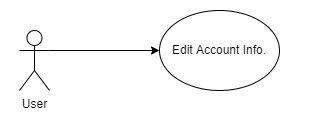
\includegraphics[height=5cm, width=0.8\textwidth]{./diagrams/Use Case/u8.png}
        \centering 
        \caption{Use Case Diagram for Edit Account Info}
        \label{fig:Usecase1}
        \end{figure}
        
    \begin{center}
        \begin{tabularx}{\textwidth}{|l|X|}
            \hline
            \textbf{ID} & UC-08 \\
            \hline
            \textbf{Name} & Edit Account Info \\
            \hline
            \textbf{Description} & User can edit their account information \\
            \hline
            \textbf{Actors} & Already User \\
            \hline
            \textbf{Triggers} & Database of that user can be updated \\
            \hline
            \textbf{Pre Conditions} & Already data of that user will be in database  \\
            \hline
            \textbf{Post Conditions} & Update the new version of their information in database \\
            \hline
            \textbf{Main Course} & Information of the User can be updated if he/she can \\
            \hline
            \textbf{Alternative Course} & Error willbe displaced by the Database \\
            \hline
            
        \end{tabularx}
    \end{center}
    \newpage 
    

    \subsubsection{UC-9: Edit Interface Preferences}
    \begin{figure}[H]
        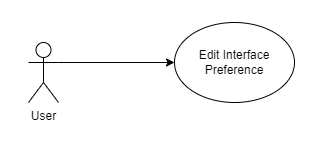
\includegraphics[height=5cm, width=0.8\textwidth]{./diagrams/Use Case/u9.png}
        \centering 
        \caption{Use Case Diagram for Edit Interface Preferences}
        \label{fig:Usecase1}
        \end{figure}
        
    \begin{center}
        \begin{tabularx}{\textwidth}{|l|X|}
            \hline
            \textbf{ID} & UC-09 \\
            \hline
            \textbf{Name} & Edit Interface Preferences \\
            \hline
            \textbf{Description} & User can edit their preferences of the UI of their dashboard \\
            \hline
            \textbf{Actors} & User \\
            \hline
            \textbf{Triggers} & User can change the primary and secondary Colors of the themes \\
            \hline
            \textbf{Pre Conditions} & Valid User \\
            \hline
            \textbf{Post Conditions} & UI preferences will be change according to User \\
            \hline
            \textbf{Main Course} & Interface preference will be changed by the user according to their preception  \\
            \hline
            \textbf{Alternative Course} & Error will be displayed it choose certain colors like black etc. \\
            \hline
            
        \end{tabularx}
    \end{center}
    \newpage
    

    \subsubsection{UC-10: Create Project}
    \begin{figure}[H]
        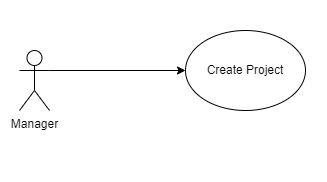
\includegraphics[height=5cm, width=0.8\textwidth]{./diagrams/Use Case/u10.png}
        \centering 
        \caption{Use Case Diagram for Create Project}
        \label{fig:Usecase1}
        \end{figure}
        
    \begin{center}
        \begin{tabularx}{\textwidth}{|l|X|}
            \hline
            \textbf{ID} & UC-10 \\
            \hline
            \textbf{Name} & Create Project \\
            \hline
            \textbf{Description} & Manager can create a project which is stored in the database with the unique id \\
            \hline
            \textbf{Actors} & Manager \\
            \hline
            \textbf{Triggers} & The Project will created in the database with unique id \\
            \hline
            \textbf{Pre Conditions} & user will be valid and Project can't created before  \\
            \hline
            \textbf{Post Conditions} & Project is created by the Manager \\
            \hline
            \textbf{Main Course} & Project is created by the manager in database \\
            \hline
            \textbf{Alternative Course} & Error will be displayed of database  \\
            \hline
            
        \end{tabularx}
    \end{center}
    
    \newpage

    \subsubsection{UC-11: Edit Project}
    \begin{figure}[H]
        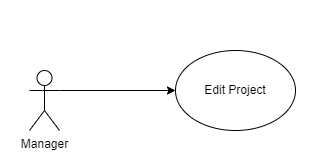
\includegraphics[height=5cm, width=0.8\textwidth]{./diagrams/Use Case/u11.png}
        \centering 
        \caption{Use Case Diagram for Edit Project}
        \label{fig:Usecase1}
        \end{figure}
        
    \begin{center}
        \begin{tabularx}{\textwidth}{|l|X|}
            \hline
            \textbf{ID} & UC-11 \\
            \hline
            \textbf{Name} & Edit Project \\
            \hline
            \textbf{Description} & The existing project will be edited by the manager if needed  \\
            \hline
            \textbf{Actors} & Manager \\
            \hline
           \textbf{Triggers} & The Information of the existing project will be updated in the database \\
            \hline
            \textbf{Pre Conditions} & Project is present already in database \\
            \hline
            \textbf{Post Conditions} & Project's Information will be updated by manager \\
            \hline
            \textbf{Main Course} & Manager can change the existing project if the requirements will be changed by the client \\
            \hline
            \textbf{Alternative Course} & Database's error will occurs \\
            \hline
            
        \end{tabularx}
    \end{center}
    \newpage
    

    \subsubsection{UC-12: Delete Project}
    \begin{figure}[H]
        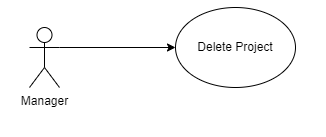
\includegraphics[height=5cm, width=0.8\textwidth]{./diagrams/Use Case/u12.png}
        \centering 
        \caption{Use Case Diagram for Delete Project}
        \label{fig:Usecase1}
        \end{figure}
        
    \begin{center}
        \begin{tabularx}{\textwidth}{|l|X|}
            \hline
            \textbf{ID} & UC-12 \\
            \hline
            \textbf{Name} & Delete Project \\
            \hline
            \textbf{Description} & The Manager will delete the existing projects Use Caseom the database \\
            \hline
            \textbf{Actors} & Managers \\
            \hline
            \textbf{Triggers} & Delete the existing project Use Caseom the database by delete event \\
            \hline
            \textbf{Pre Conditions} & Project will be in the database which Manager will be deleted \\
            \hline
            \textbf{Post Conditions} & Project is deletedby the the manager \\
            \hline
            \textbf{Main Course} & The manager will delete the exiting project which is presnet in database \\
            \hline
            \textbf{Alternative Course} & Error will be displayed \\
            \hline
            
        \end{tabularx}
    \end{center}
    \newpage
    

    \subsubsection{UC-13: Add Developer}
    \begin{figure}[H]
        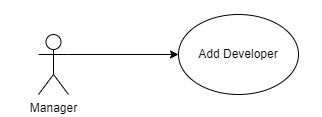
\includegraphics[height=5cm, width=0.8\textwidth]{./diagrams/Use Case/u13.png}
        \centering 
        \caption{Use Case Diagram for Add Developer}
        \label{fig:Usecase1}
        \end{figure}
        
    \begin{center}
        \begin{tabularx}{\textwidth}{|l|X|}
            \hline
            \textbf{ID} & UC-13 \\
            \hline
            \textbf{Name} & Add Developer \\
            \hline
            \textbf{Description} & The Manager will assign the developer of the company which is part of that Project \\
            \hline
            \textbf{Actors} & Managers \\
            \hline
            \textbf{Triggers} & Developer list will be shown to manager and manager will add the relevant developer \\
            \hline
            \textbf{Pre Conditions} & Developer and project will be added \\
            \hline
            \textbf{Post Conditions} & Developer will be added in the specific project \\
            \hline
            \textbf{Main Course} & To view the new upcoming project and take the decision of developer in project, Manager will added the developer in the project \\
            \hline
            \textbf{Alternative Course} & Error will be displayed \\
            \hline
            
        \end{tabularx}
    \end{center}
    
    \newpage

    \subsubsection{UC-14: Remove Developer}
    \begin{figure}[H]
        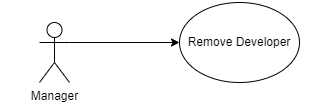
\includegraphics[height=5cm, width=0.8\textwidth]{./diagrams/Use Case/u14.png}
        \centering 
        \caption{Use Case Diagram for Remove Developer}
        \label{fig:Usecase1}
        \end{figure}
        
    \begin{center}
        \begin{tabularx}{\textwidth}{|l|X|}
            \hline
            \textbf{ID} & UC-14 \\
            \hline
            \textbf{Name} & Remove Developer \\
            \hline
            \textbf{Description} & The manager can remove the developer after developer performs their duties \\
            \hline
            \textbf{Actors} & Manager \\
            \hline
           \textbf{Triggers} & Manager will remove the developer in the project anytime. \\
            \hline
            \textbf{Pre Conditions} & Developer will be added in that project \\
            \hline
            \textbf{Post Conditions} & developer is no more the part of the project \\
            \hline
            \textbf{Main Course} & Manager can manage the availabilty of the developer whenever he enter in the project or when he exits. \\
            \hline
            \textbf{Alternative Course} & Error will be displayed \\
            \hline
            
        \end{tabularx}
    \end{center}
    \newpage
    

    \subsubsection{UC-15: Edit Developer Permission}
    \begin{figure}[H]
        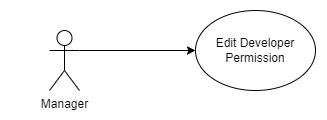
\includegraphics[height=5cm, width=0.8\textwidth]{./diagrams/Use Case/u15.png}
        \centering 
        \caption{Use Case Diagram for Edit Developer Permission}
        \label{fig:Usecase1}
        \end{figure}
        
    \begin{center}
        \begin{tabularx}{\textwidth}{|l|X|}
            \hline
            \textbf{ID} & UC-15 \\
            \hline
            \textbf{Name} & Edit Developer Permission \\
            \hline
            \textbf{Description} & The Manager can edit the role of the developer in the project \\
            \hline
            \textbf{Actors} & Managers \\
            \hline
            \textbf{Triggers} & Manager can edit the preference of the developer \\
            \hline
            \textbf{Pre Conditions} & Developer must have the part of the project \\
            \hline
            \textbf{Post Conditions} & Developer's Role will changed by the manager \\
            \hline
            \textbf{Main Course} & The Developer can change the role of the developer as he needs him in the project \\
            \hline
            \textbf{Alternative Course} & Error will be dislpayed by the database \\
            \hline
            
        \end{tabularx}
    \end{center}
    \newpage
    

    \subsubsection{UC-16: Calculate UCP}
    \begin{figure}[H]
        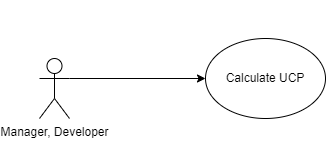
\includegraphics[height=5cm, width=0.8\textwidth]{./diagrams/Use Case/u16.png}
        \centering 
        \caption{Use Case Diagram for Calculate UCP}
        \label{fig:Usecase1}
        \end{figure}
        
    \begin{center}
        \begin{tabularx}{\textwidth}{|l|X|}
            \hline
            \textbf{ID} & UC-16 \\
            \hline
            \textbf{Name} & Calculate UCP \\
            \hline
            \textbf{Description} & Calculate the effort estimation of project via mean of UCP method \\
            \hline
            \textbf{Actors} & Manager , Developers \\
            \hline
            \textbf{Triggers} & The effort will calculted by UCP formula \\
            \hline
            \textbf{Pre Conditions} & The Project Use cases' information are inserted already \\
            \hline
            \textbf{Post Conditions} & Calculated Effort are given by UCP method  \\
            \hline
            \textbf{Main Course} & To find the Effort Estimation by UCP method of the entire project by the help of their use cases \\
            \hline
            \textbf{Alternative Course} & Error will displayed \\
            \hline
            
        \end{tabularx}
    \end{center}
    
    \newpage

    \subsubsection{UC-17: Get Machine Learning Estimation}
    \begin{figure}[H]
        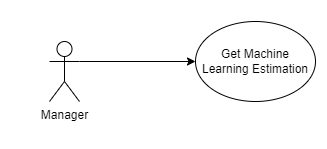
\includegraphics[height=5cm, width=0.8\textwidth]{./diagrams/Use Case/u17.png}
        \centering 
        \caption{Use Case Diagram for Get Machine Learning Estimation}
        \label{fig:Usecase1}
        \end{figure}
        
    \begin{center}
        \begin{tabularx}{\textwidth}{|l|X|}
            \hline
            \textbf{ID} & UC-17 \\
            \hline
            \textbf{Name} & Get Machine Learning Estimation \\
            \hline
            \textbf{Description} & Calculate the effort estimation of project via trained Machine Learning module \\
            \hline
            \textbf{Actors} & Manager  \\
            \hline
            \textbf{Triggers} & The effort will calculted by UCP formula \\
            \hline
            \textbf{Pre Conditions} & The Project Use cases' information are inserted already \\
            \hline
            \textbf{Post Conditions} & Calculated Effort are given by UCP method  \\
            \hline
            \textbf{Main Course} & To find the Effort Estimation by UCP method of the entire project by the help of their use cases \\
            \hline
            \textbf{Alternative Course} & Error will displayed \\
            \hline
            
        \end{tabularx}
    \end{center}
    \newpage
    

    \subsubsection{UC-18: Manual Estimate Round}
    \begin{figure}[H]
        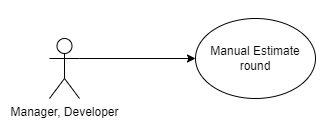
\includegraphics[height=5cm, width=0.8\textwidth]{./diagrams/Use Case/u18.png}
        \centering 
        \caption{Use Case Diagram for Manual Estimate Round}
        \label{fig:Usecase1}
        \end{figure}
        
    \begin{center}
        \begin{tabularx}{\textwidth}{|l|X|}
            \hline
            \textbf{ID} & UC-18 \\
            \hline
            \textbf{Name} & Manual Estimate Round \\
            \hline
            \textbf{Description} & Calculate the effort estimation of project via Manual Estimation where the developer and experts will estimate the project while round \\
            \hline
            \textbf{Actors} & developers, manager \\
            \hline
            \textbf{Triggers} & The Effort will calculated by Manual technique \\
            \hline
            \textbf{Pre Conditions} & Developers were added by manager  in the project \\
            \hline
            \textbf{Post Conditions} & The effort will calculated after the many rounds of the experts' discussions  \\
            \hline
            \textbf{Main Course} & To find the Effort estimation by Manual technique by many rounds \\
            \hline
            \textbf{Alternative Course} & Error will displayed \\
            \hline
            
        \end{tabularx}
    \end{center}
    
    \newpage

    \subsubsection{UC-19: Estimation Bar}
    \begin{figure}[H]
        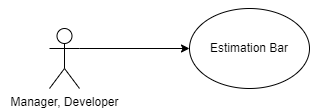
\includegraphics[height=5cm, width=0.8\textwidth]{./diagrams/Use Case/u19.png}
        \centering 
        \caption{Use Case Diagram for Estimation Bar}
        \label{fig:Usecase1}
        \end{figure}
        
    \begin{center}
        \begin{tabularx}{\textwidth}{|l|X|}
            \hline
            \textbf{ID} & UC-19 \\
            \hline
            \textbf{Name} & Estimation Bar \\
            \hline
            \textbf{Description} & All Estimation will be shown in the form of graphs \\
            \hline
            \textbf{Actors} & Manager , Developer \\
            \hline
            \textbf{Triggers} & The Estimate will be generated by the experts' round discussion \\
            \hline
            \textbf{Pre Conditions} & The estimation will be measured before that step  \\
            \hline
            \textbf{Post Conditions} & The charts will be appeared \\
            \hline
            \textbf{Main Course} & Estimation will be deliver in bar that anyone will be see and clearly judge the estimation of the project \\
            \hline
            \textbf{Alternative Course} & Error wil be displayed \\
            \hline
            
        \end{tabularx}
    \end{center}
    \newpage

    \subsubsection{UC-20: Logout}
    \begin{figure}[H]
        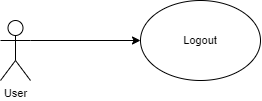
\includegraphics[height=5cm, width=0.8\textwidth]{./diagrams/Use Case/logout.png}
        \centering 
        \caption{Use Case Diagram for logout}
        \label{Usecase1}
        \end{figure}
        
    
    \begin{center}
        \begin{tabularx}{\textwidth}{|l|X|}
            \hline
            \textbf{ID} & UC-20 \\
            \hline
            \textbf{Name} & Logout \\
            \hline
            \textbf{Description} & For ending their session with the system \\
            \hline
            \textbf{Actors} & Already User \\
            \hline
            \textbf{Triggers} & Must be login and the pop up window is appeared for the confirmation. \\
            \hline
            \textbf{Pre Conditions} & They must have a account \\
            \hline
            \textbf{Post Conditions} & System display the main page  \\
            \hline
            \textbf{Main Course} & System logged out and show a pop up again with the message of "Sucessfully logged out" \\
            \hline
            \textbf{Alternative Course} & Error due to invalid details \\
            \hline
            
        \end{tabularx}
    \end{center}
    \newpage
    

    

  

% Chapter 4 Design
%
\section{Design}

\vspace{20mm}



\begin{abstract}

    This chapter is dedicated to representing the design of the system through a variety of different UML diagrams.


\end{abstract}

\vspace{20mm}

\large{\textbf{Outline}}

\begin{center}
    \begin{itemize}
        \item Architecture Diagram
        \item Entity Relationship Diagram
        \item Data Dictionary Diagram
        \item Data Flow Diagram
        \item Activity Diagram
        \item Sequence Diagram
        \item Collaboration Diagram
        \item State Transition Diagram
        \item Component Diagram
        \item Deployment Diagram
    \end{itemize}
\end{center}
\pagebreak


% Architecture Diagram
\subsection{Architecture Diagram}
\begin{figure}[H]
    \centering
    \caption{Architecture Diagram}
    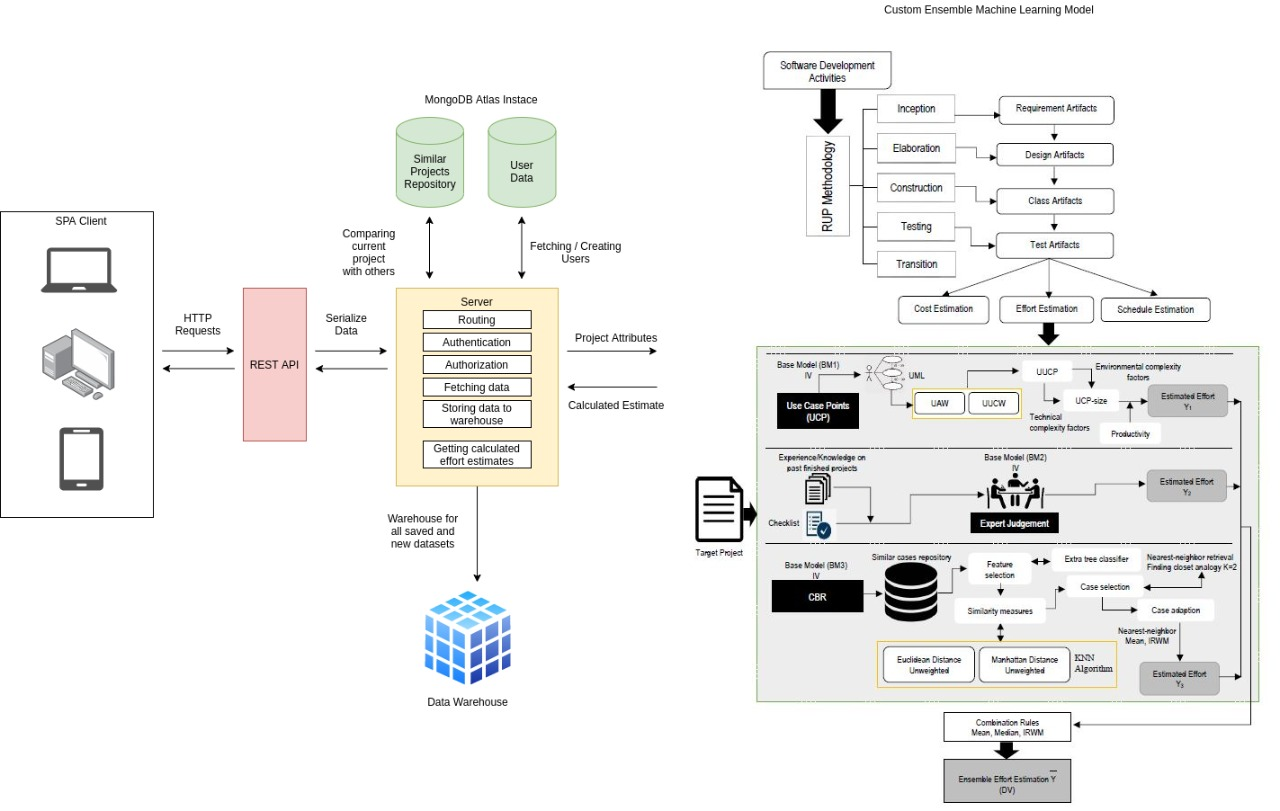
\includegraphics[scale=0.4]{./diagrams/architecture-diagram.jpeg}
    \label{fig:arch-diag}

\end{figure}


% Entity Relationship Diagram
\subsection{Entity Relationship Diagram}
\begin{figure}[H]
    \centering
    \caption{Entity Relationship Diagram}
    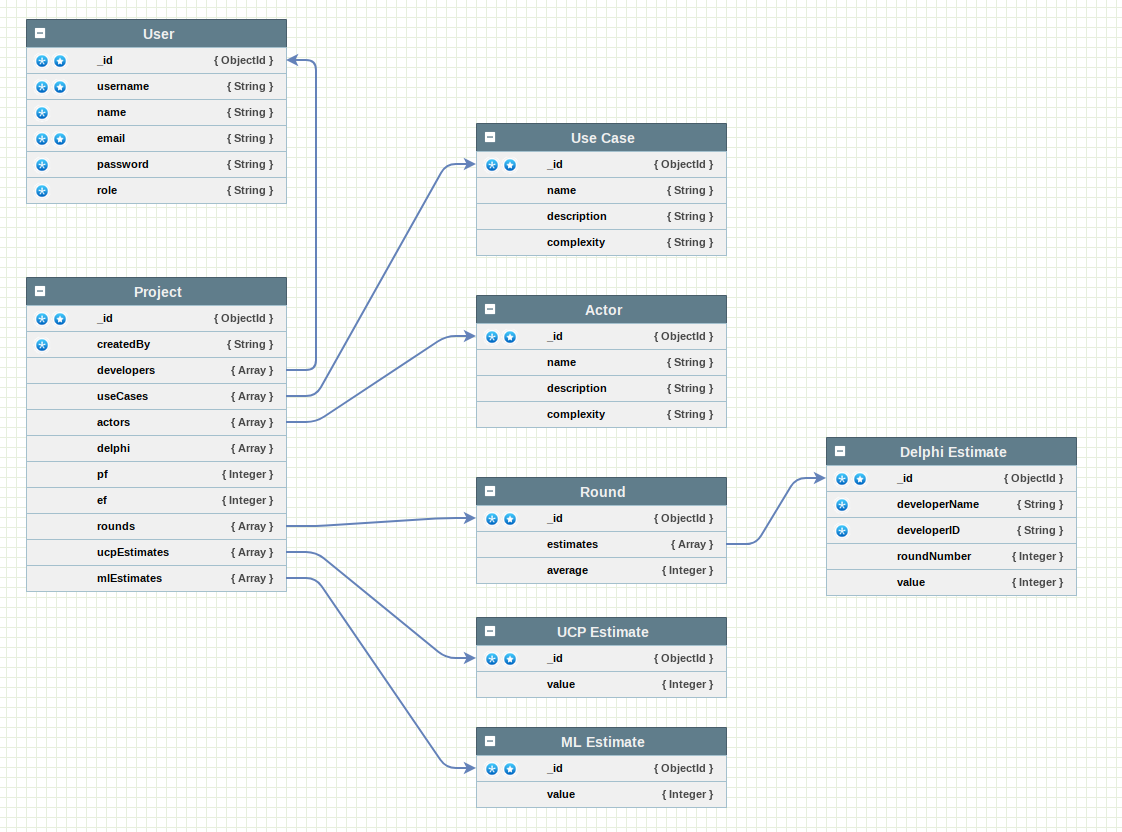
\includegraphics[scale=0.4]{./diagrams/ERD.png}
    \label{fig:er-diag}

\end{figure}


% Data Dictionary Diagram

\subsection{Data Dictionary Diagram}


\begin{figure}[H]
    \centering
    \caption{Data Dictionary Diagram 1}
    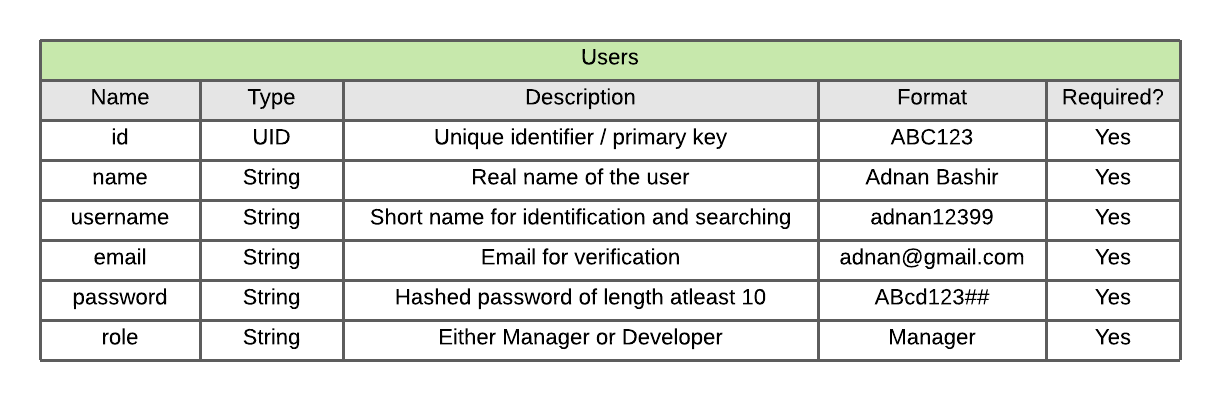
\includegraphics[scale=0.7]{./diagrams/data-dictionary/dd-1.png}
    \label{fig:dd-diag-1}

\end{figure}


\begin{figure}[H]
    \centering
    \caption{Data Dictionary Diagram 2}
    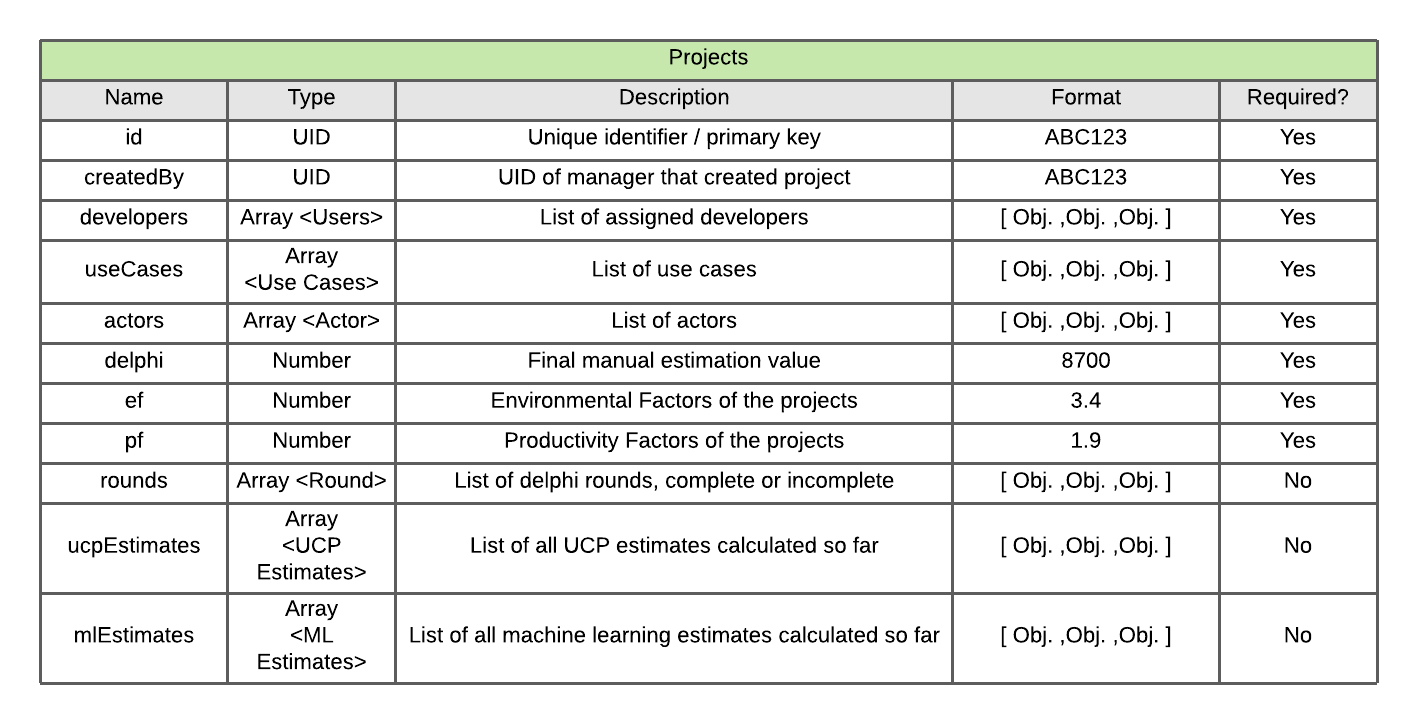
\includegraphics[scale=0.7]{./diagrams/data-dictionary/dd-2.png}
    \label{fig:dd-diag-2}
\end{figure}


\begin{figure}[H]
    \centering
    \caption{Data Dictionary Diagram 3}
    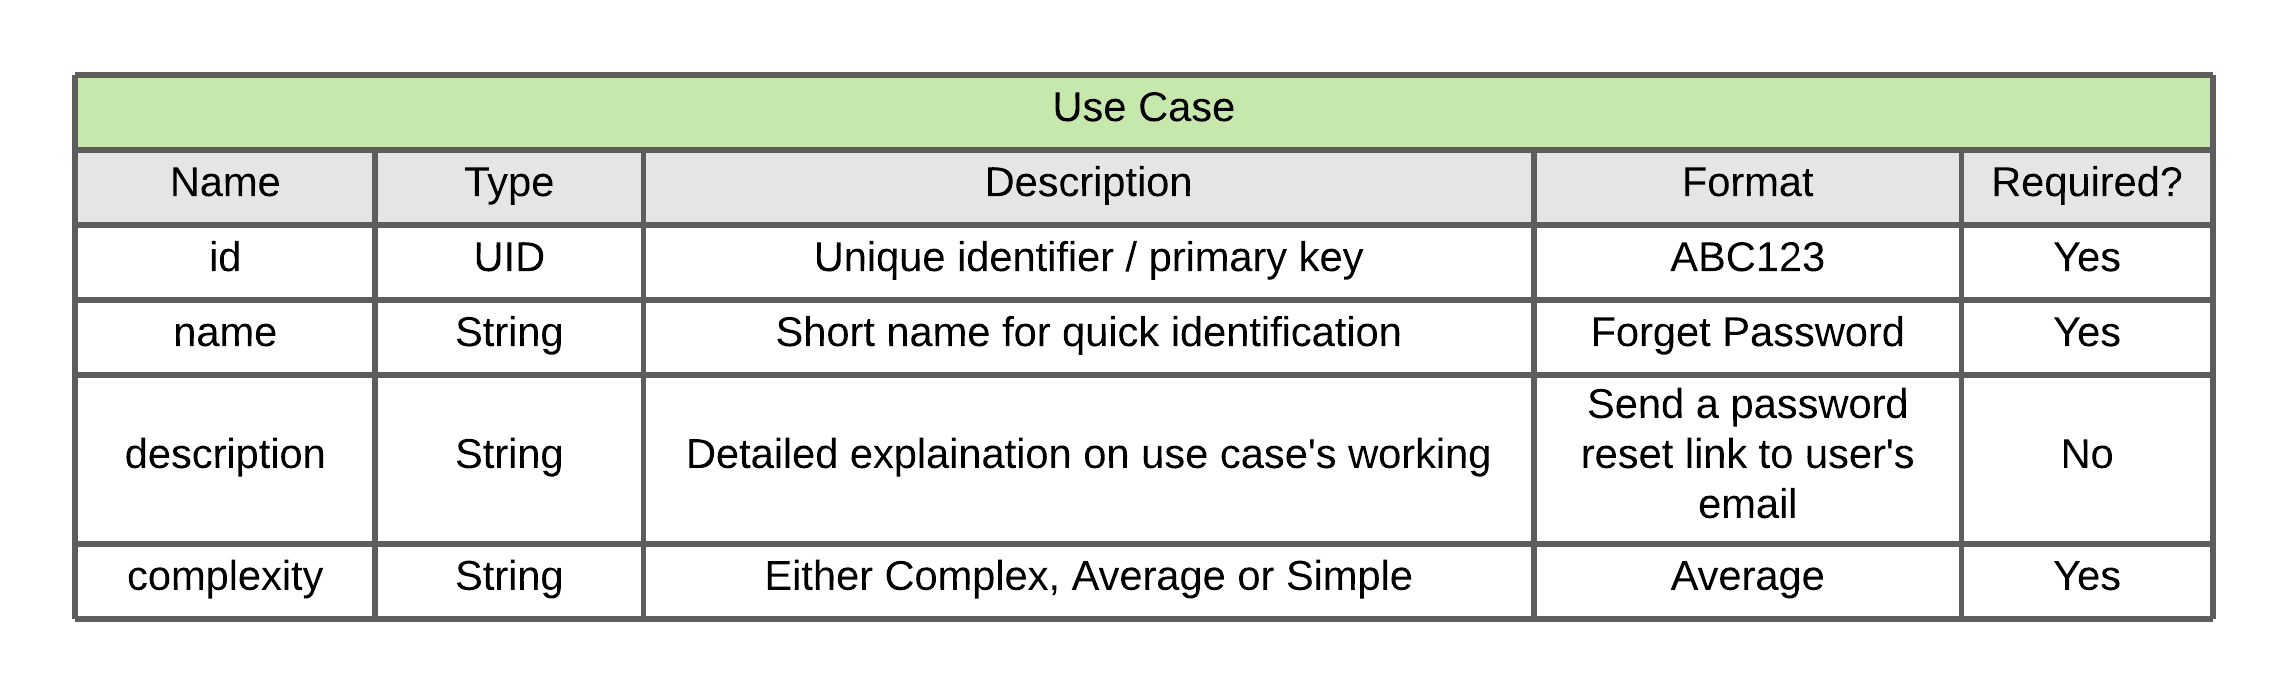
\includegraphics[scale=0.7]{./diagrams/data-dictionary/dd-3.png}
    \label{fig:dd-diag-3}

\end{figure}


\begin{figure}[H]
    \centering
    \caption{Data Dictionary Diagram 4}
    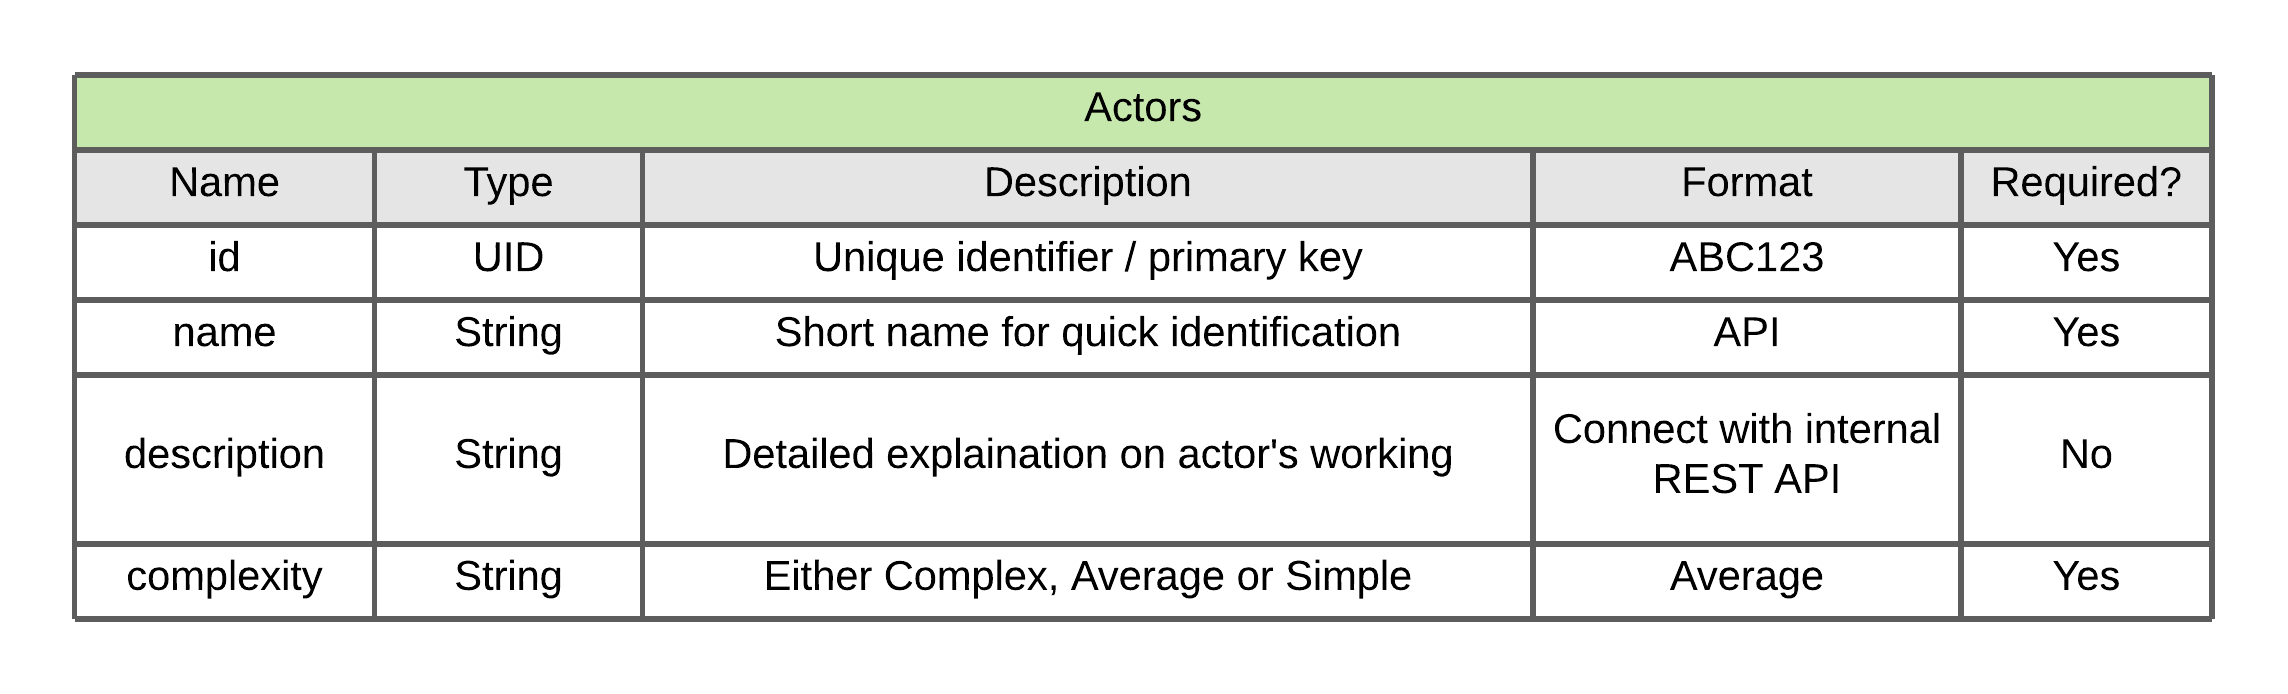
\includegraphics[scale=0.7]{./diagrams/data-dictionary/dd-4.png}
    \label{fig:dd-diag-4}

\end{figure}


\begin{figure}[H]
    \centering
    \caption{Data Dictionary Diagram 5}
    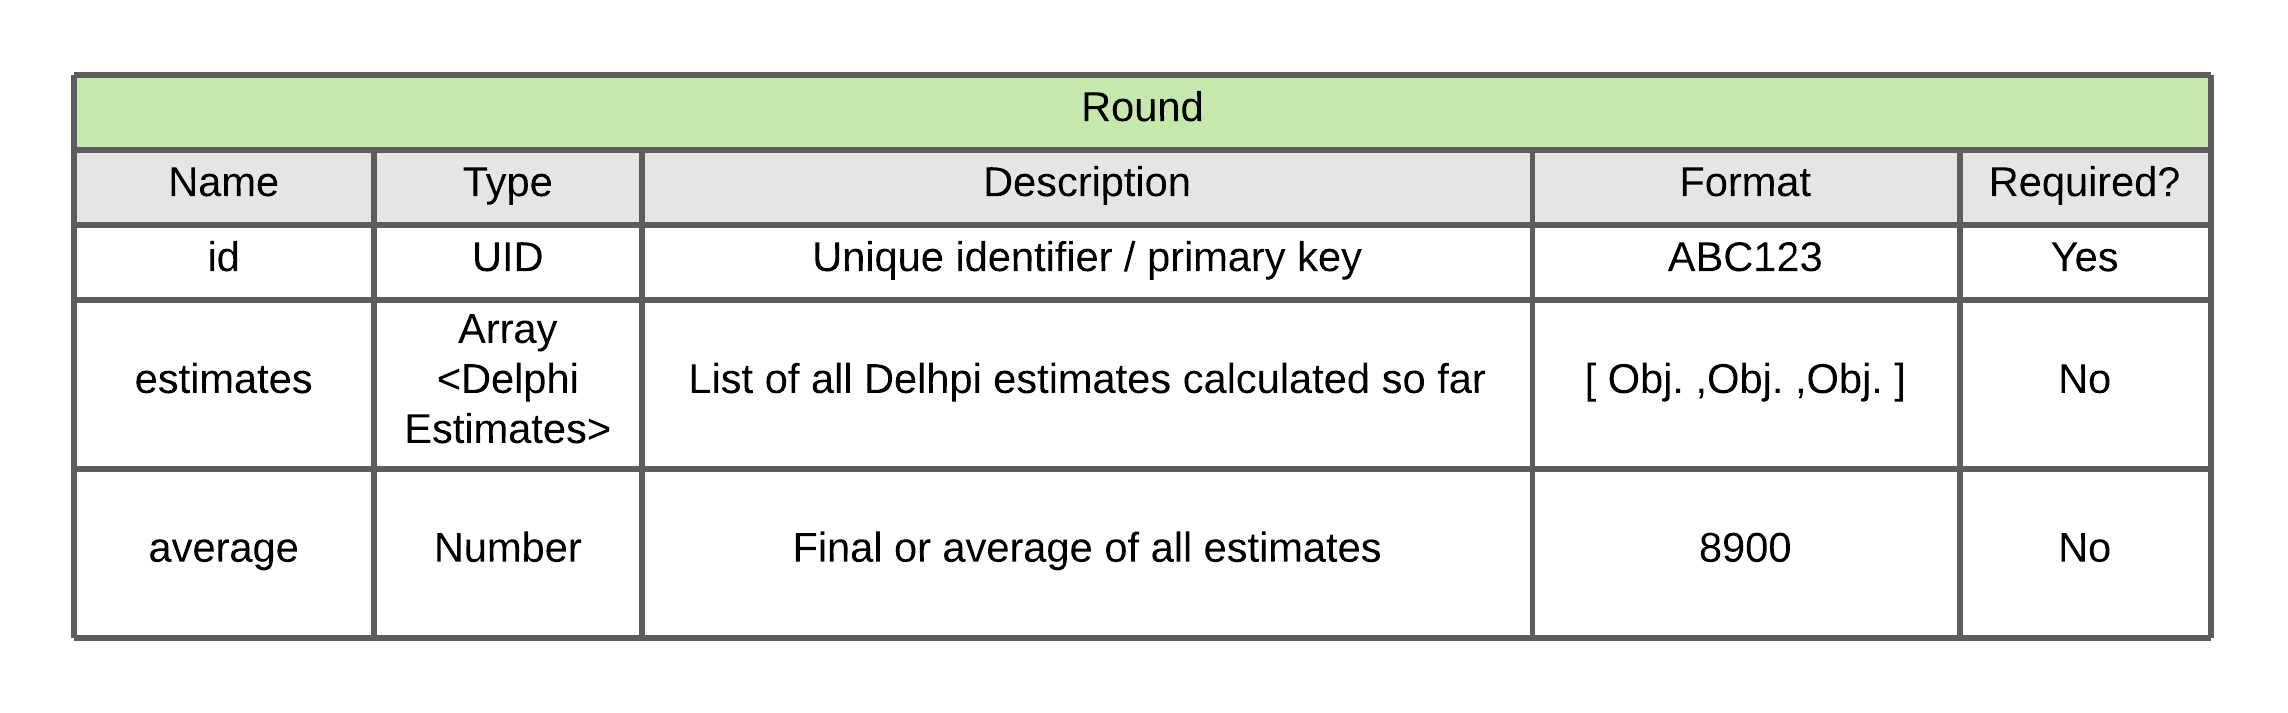
\includegraphics[scale=0.7]{./diagrams/data-dictionary/dd-5.png}
    \label{fig:dd-diag-5}

\end{figure}



\begin{figure}[H]
    \centering
    \caption{Data Dictionary Diagram 6}
    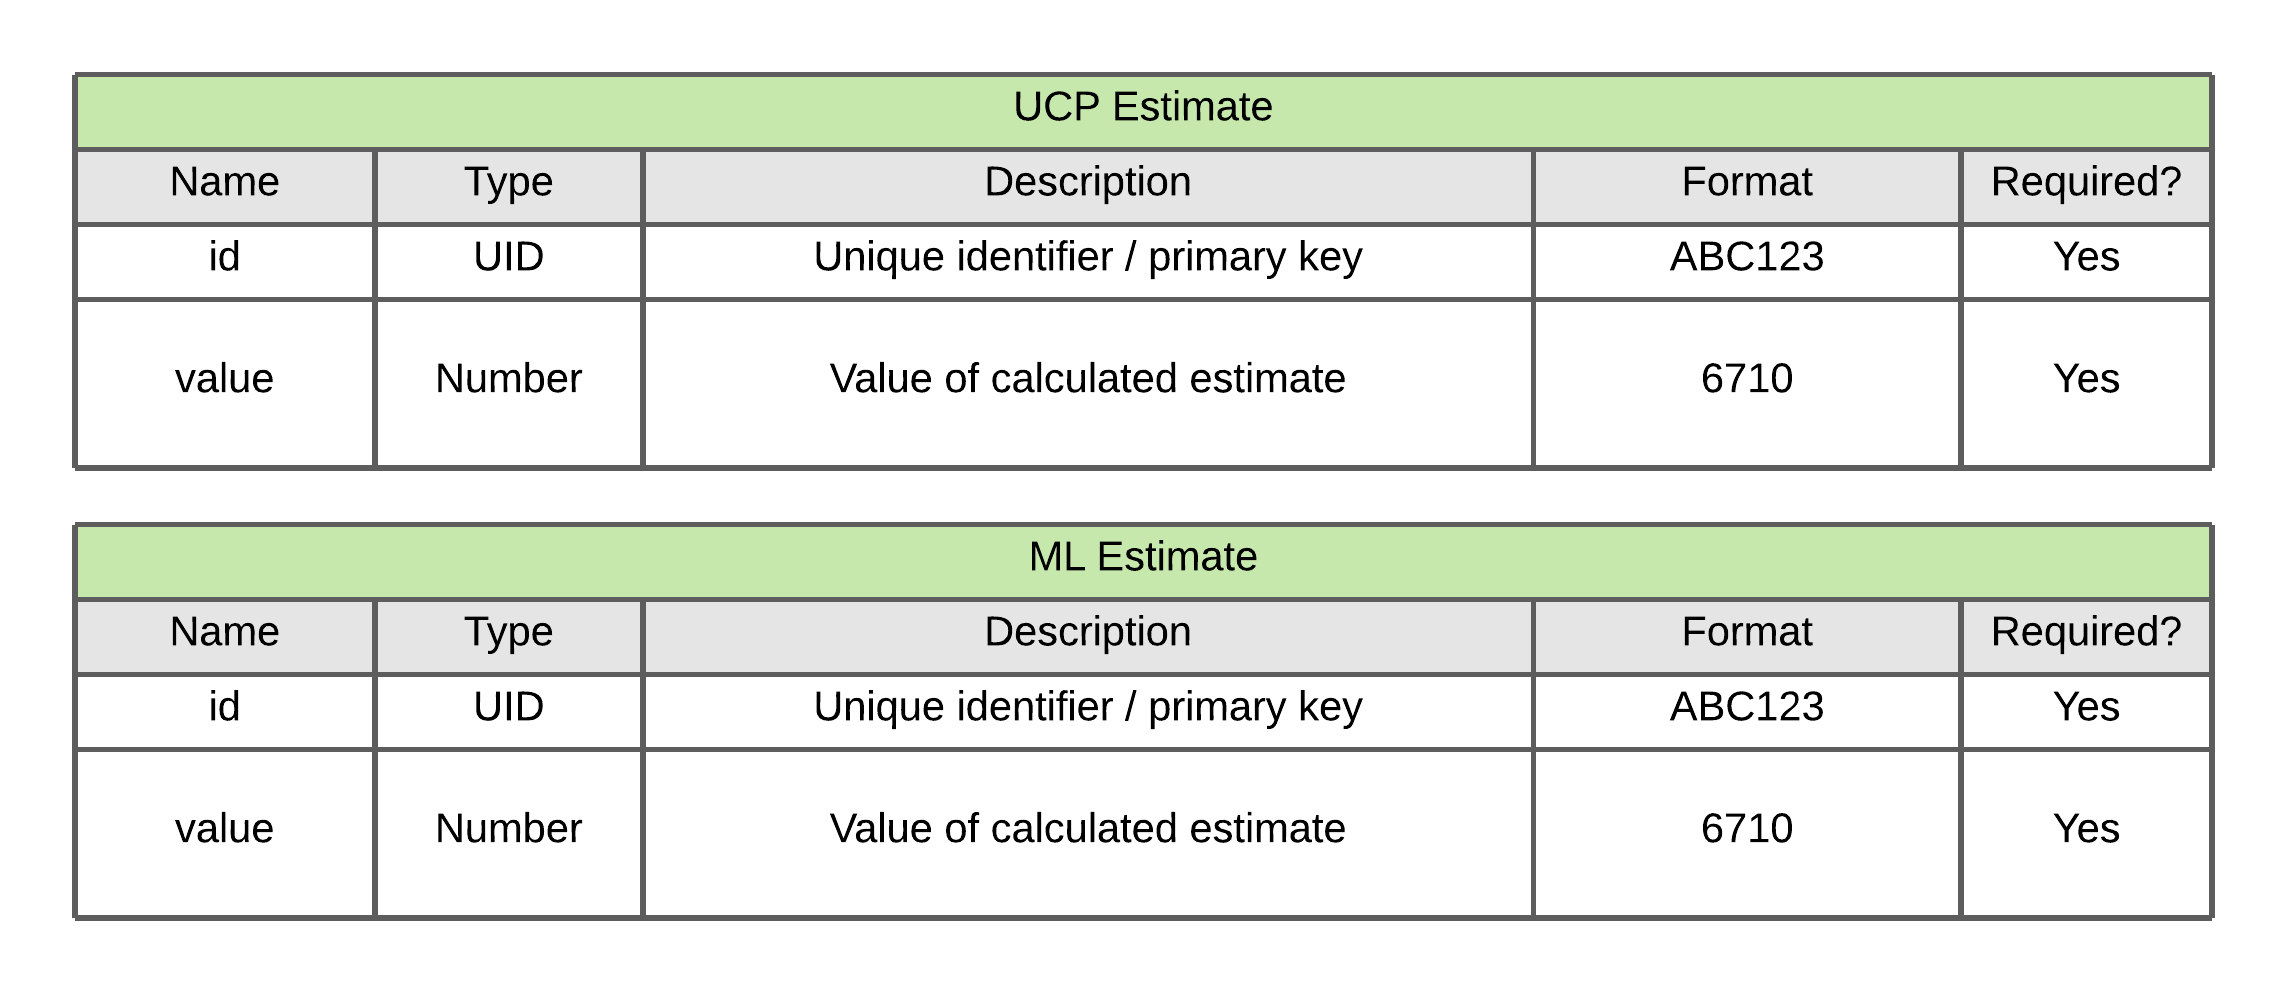
\includegraphics[scale=0.7]{./diagrams/data-dictionary/dd-6.png}
    \label{fig:dd-diag-6}
\end{figure}

% Data Flow Diagram
% Data Flow Diagram
\subsection{Data Flow Diagram}

\subsubsection{Level 1}

\begin{figure}[H]
    \centering
    \caption{Data Flow Diagram 1}
    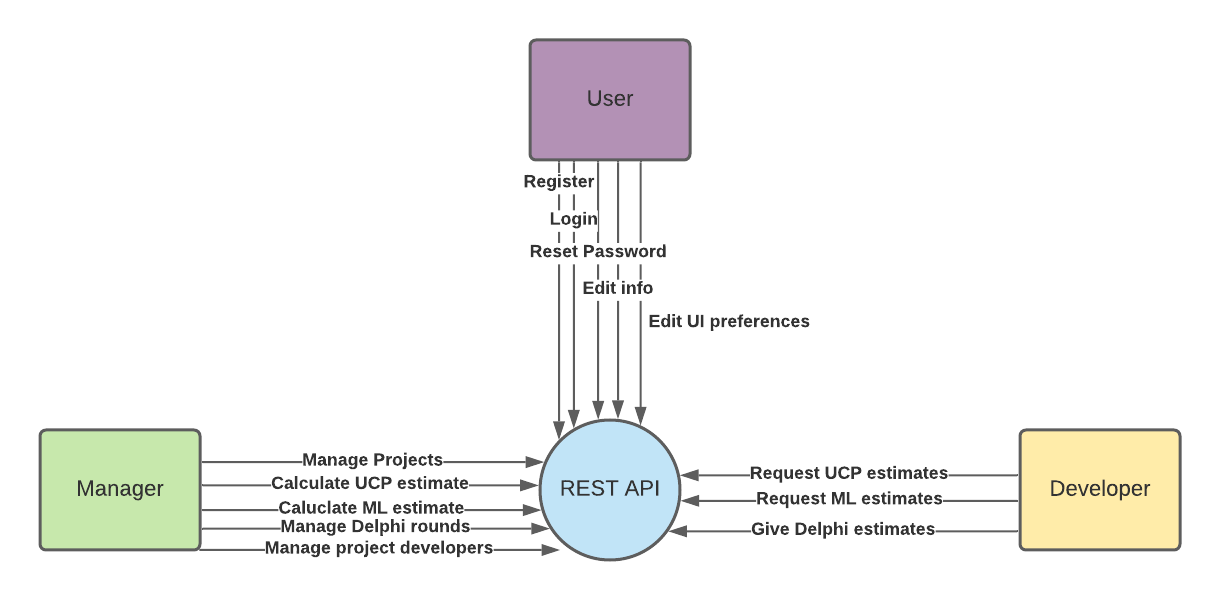
\includegraphics[scale=0.7]{./diagrams/data-flow/df-1.png}
    \label{fig:df-diag-1}
\end{figure}


\subsubsection{Level 2}
\begin{figure}[H]
    \centering
    \caption{Data Flow Diagram 2}
    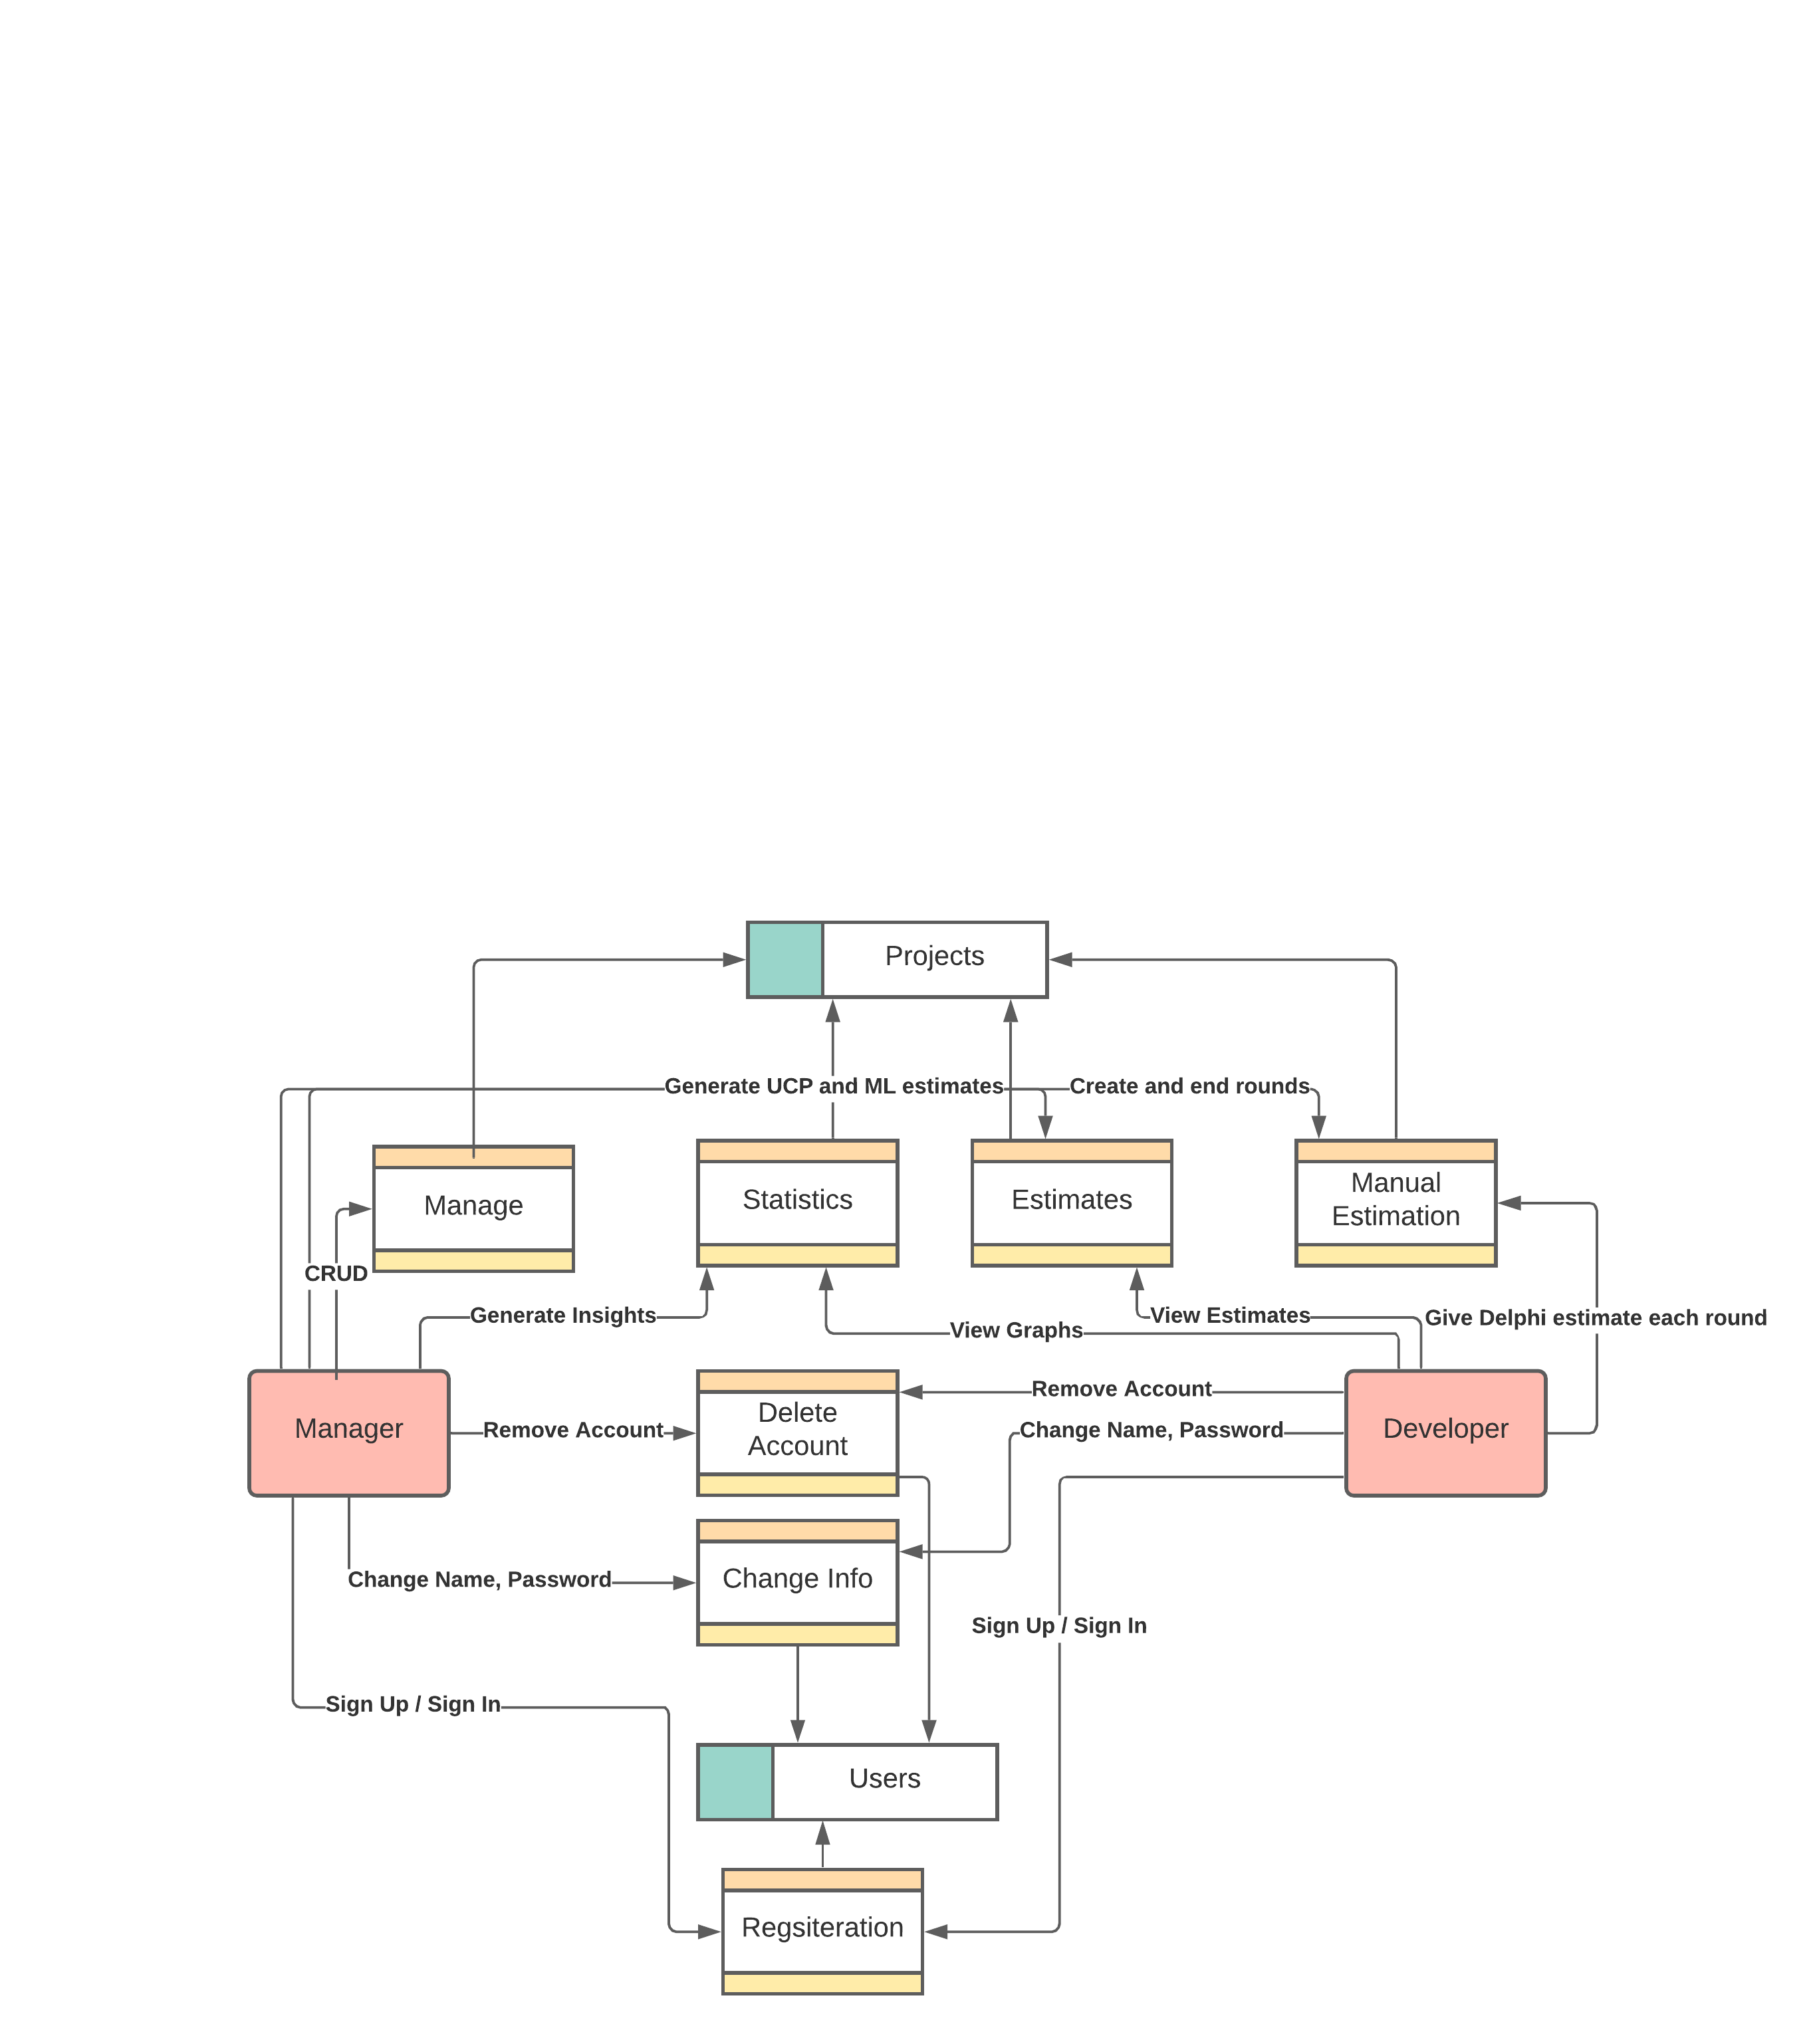
\includegraphics[scale=0.7]{./diagrams/data-flow/df-2.png}
    \label{fig:df-diag-2}
\end{figure}


% Activity Diagram
\subsection{Activity Diagram}

\begin{figure}[H]
    \centering
    \caption{Activity Diagram 1}
    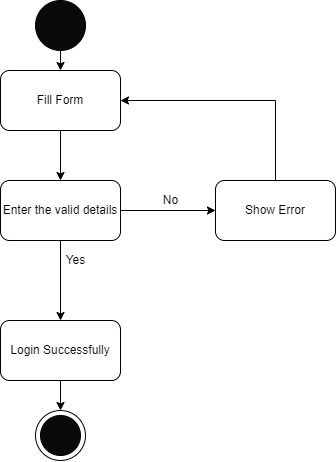
\includegraphics[scale=0.5]{./diagrams/Activity Diagram/ad-01.png}
    \label{fig:act-01}

\end{figure}


\begin{figure}[H]
    \centering
    \caption{Activity Diagram 2}
    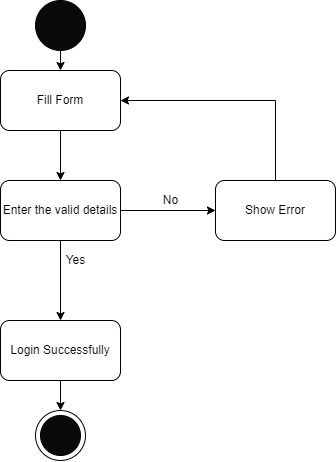
\includegraphics[scale=0.5]{./diagrams/Activity Diagram/ad-02.png}
    \label{fig:act-02}

\end{figure}


\begin{figure}[H]
    \centering
    \caption{Activity Diagram 3}
    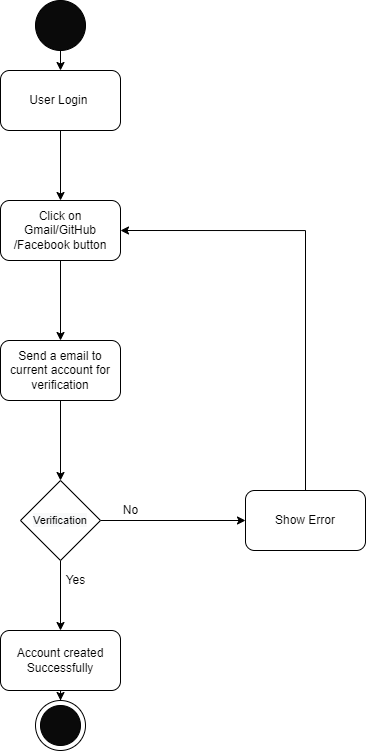
\includegraphics[scale=0.5]{./diagrams/Activity Diagram/ad-03.png}
    \label{fig:act-03}

\end{figure}


\begin{figure}[H]
    \centering
    \caption{Activity Diagram 4}
    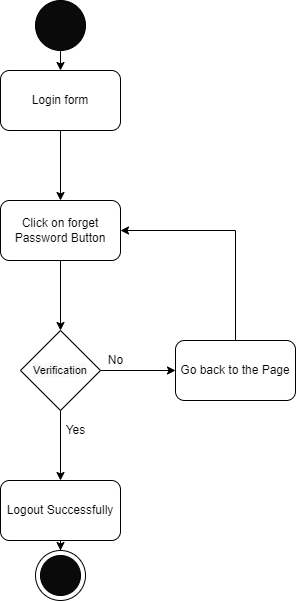
\includegraphics[scale=0.5]{./diagrams/Activity Diagram/ad-04.png}
    \label{fig:act-04}

\end{figure}


\begin{figure}[H]
    \centering
    \caption{Activity Diagram 5}
    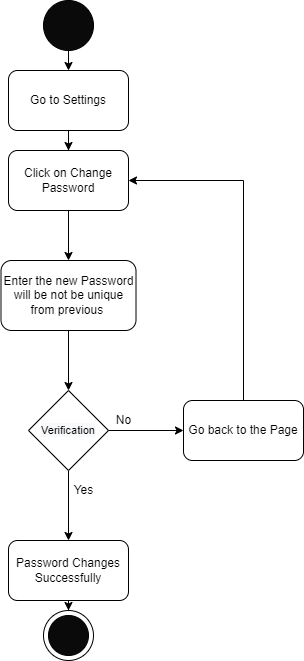
\includegraphics[scale=0.5]{./diagrams/Activity Diagram/ad-05.png}
    \label{fig:act-05}

\end{figure}


\begin{figure}[H]
    \centering
    \caption{Activity Diagram 6}
    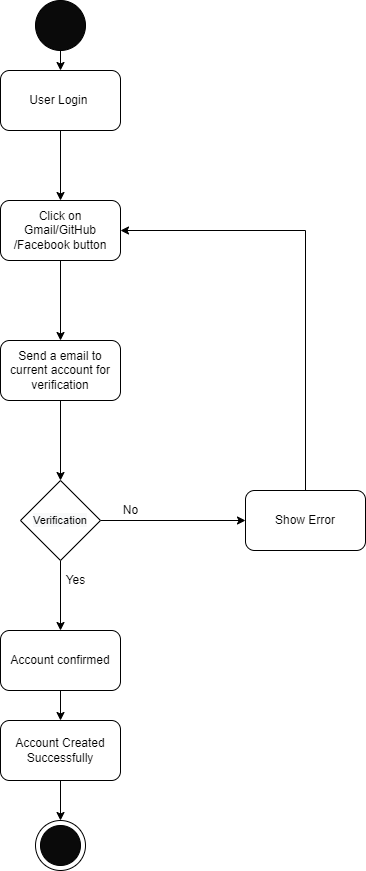
\includegraphics[scale=0.5]{./diagrams/Activity Diagram/ad-06.png}
    \label{fig:act-06}

\end{figure}


\begin{figure}[H]
    \centering
    \caption{Activity Diagram 7}
    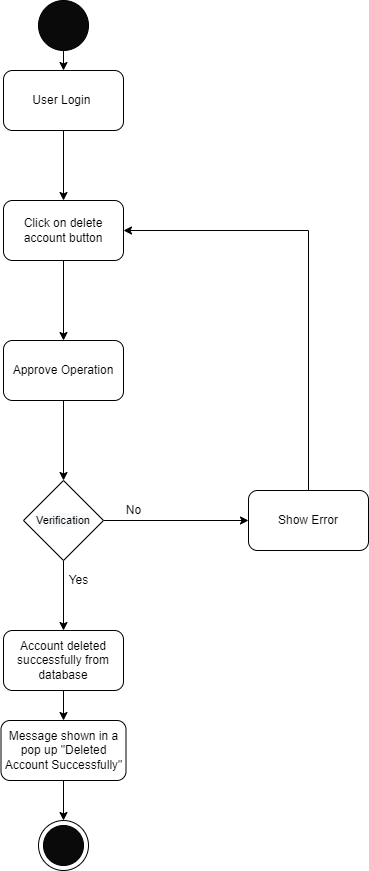
\includegraphics[scale=0.5]{./diagrams/Activity Diagram/ad-07.png}
    \label{fig:act-07}

\end{figure}


\begin{figure}[H]
    \centering
    \caption{Activity Diagram 8}
    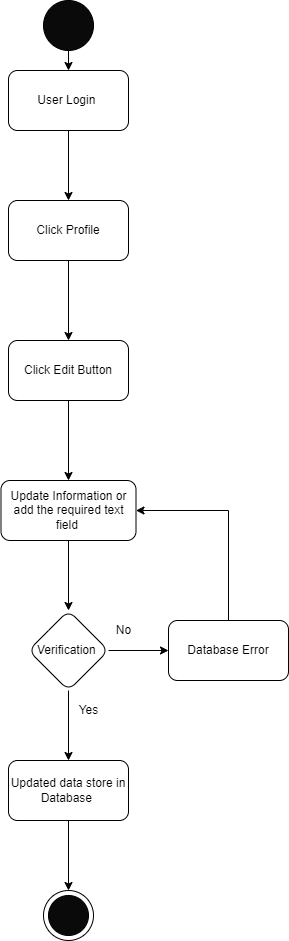
\includegraphics[scale=0.5]{./diagrams/Activity Diagram/ad-08.png}
    \label{fig:act-08}

\end{figure}


\begin{figure}[H]
    \centering
    \caption{Activity Diagram 9}
    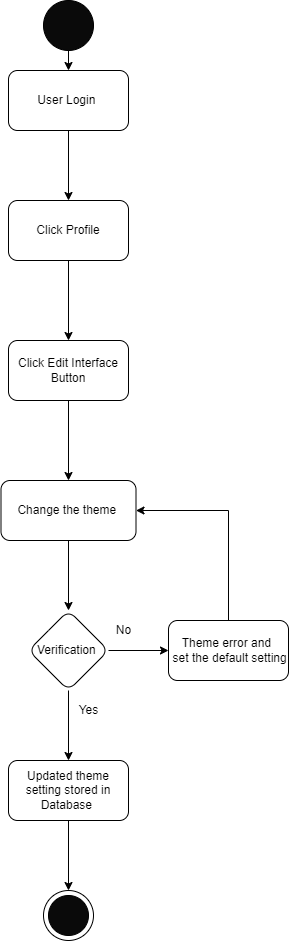
\includegraphics[scale=0.5]{./diagrams/Activity Diagram/ad-09.png}
    \label{fig:act-09}

\end{figure}


\begin{figure}[H]
    \centering
    \caption{Activity Diagram 10}
    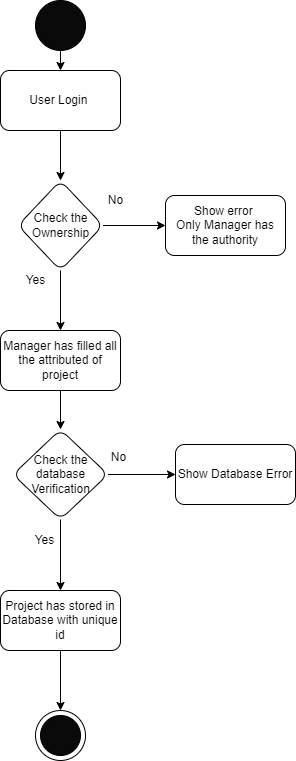
\includegraphics[scale=0.5]{./diagrams/Activity Diagram/ad-10.png}
    \label{fig:act-10}

\end{figure}


\begin{figure}[H]
    \centering
    \caption{Activity Diagram 11}
    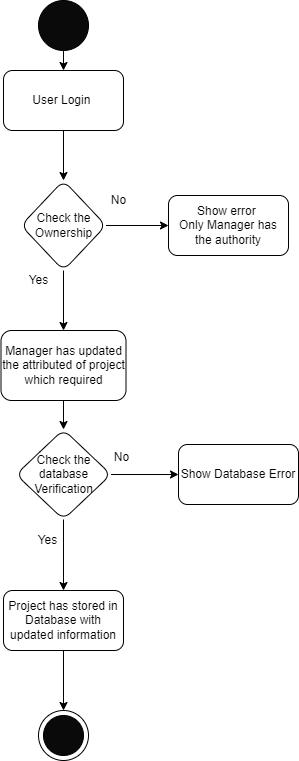
\includegraphics[scale=0.5]{./diagrams/Activity Diagram/ad-11.png}
    \label{fig:act-11}

\end{figure}


\begin{figure}[H]
    \centering
    \caption{Activity Diagram 12}
    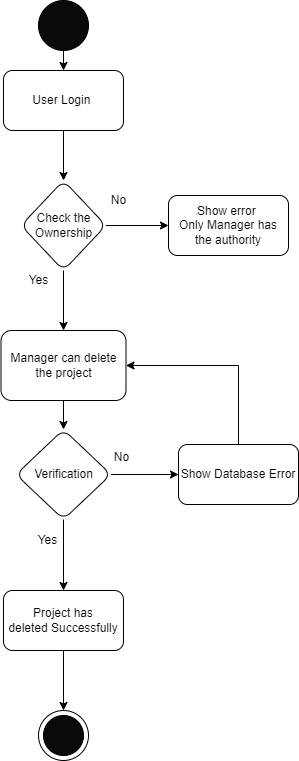
\includegraphics[scale=0.5]{./diagrams/Activity Diagram/ad-12.png}
    \label{fig:act-12}

\end{figure}


\begin{figure}[H]
    \centering
    \caption{Activity Diagram 13}
    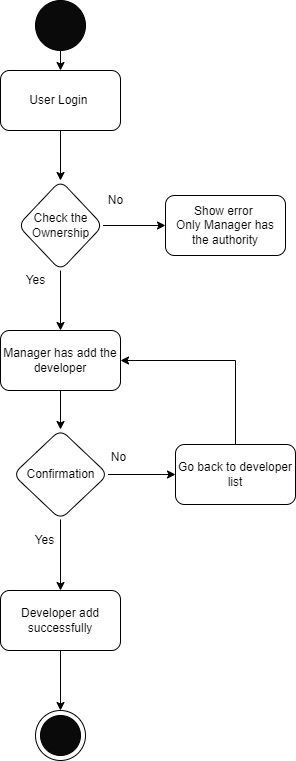
\includegraphics[scale=0.5]{./diagrams/Activity Diagram/ad-13.png}
    \label{fig:act-13}

\end{figure}


\begin{figure}[H]
    \centering
    \caption{Activity Diagram 14}
    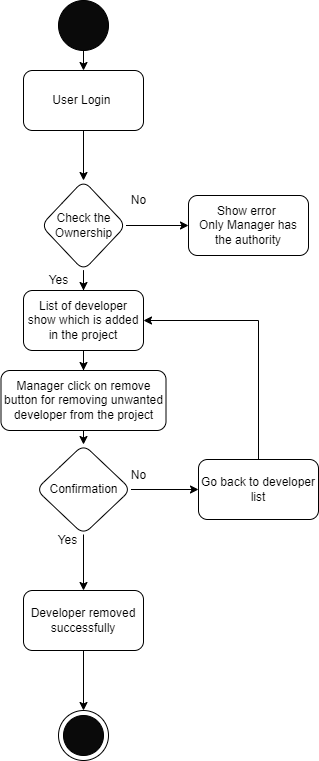
\includegraphics[scale=0.5]{./diagrams/Activity Diagram/ad-14.png}
    \label{fig:act-14}

\end{figure}


\begin{figure}[H]
    \centering
    \caption{Activity Diagram 15}
    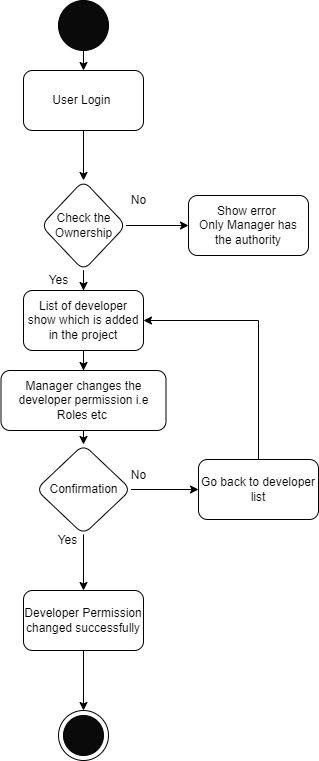
\includegraphics[scale=0.5]{./diagrams/Activity Diagram/ad-15.png}
    \label{fig:act-15}

\end{figure}


\begin{figure}[H]
    \centering
    \caption{Activity Diagram 16}
    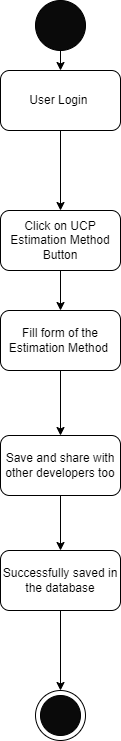
\includegraphics[scale=0.5]{./diagrams/Activity Diagram/ad-16.png}
    \label{fig:act-16}

\end{figure}


\begin{figure}[H]
    \centering
    \caption{Activity Diagram 17}
    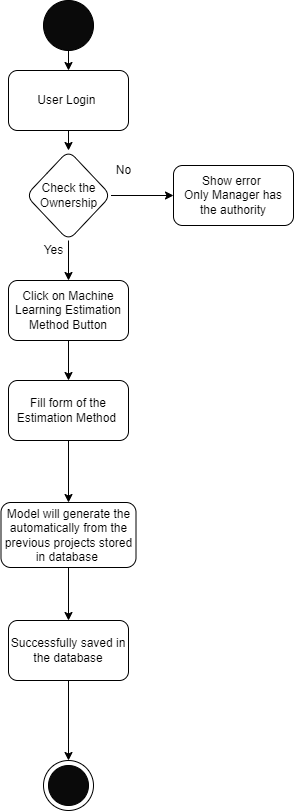
\includegraphics[scale=0.5]{./diagrams/Activity Diagram/ad-17.png}
    \label{fig:act-17}

\end{figure}


\begin{figure}[H]
    \centering
    \caption{Activity Diagram 18}
    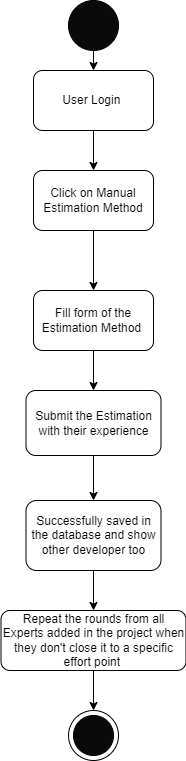
\includegraphics[scale=0.5]{./diagrams/Activity Diagram/ad-18.png}
    \label{fig:act-18}

\end{figure}


\begin{figure}[H]
    \centering
    \caption{Activity Diagram 19}
    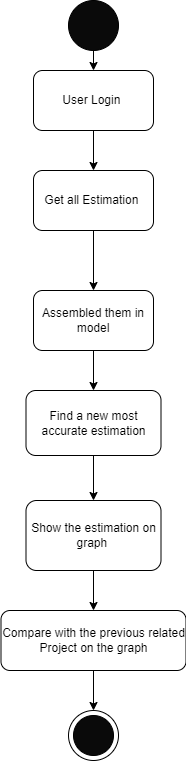
\includegraphics[scale=0.5]{./diagrams/Activity Diagram/ad-19.png}
    \label{fig:act-19}

\end{figure}


\begin{figure}[H]
    \centering
    \caption{Activity Diagram 1}
    \includegraphics[scale=0.5]{./diagrams/Activity Diagram/ad-01.png}
    \label{fig:act-01}

\end{figure}


\begin{figure}[H]
    \centering
    \caption{Activity Diagram 2}
    \includegraphics[scale=0.5]{./diagrams/Activity Diagram/ad-02.png}
    \label{fig:act-02}

\end{figure}


\begin{figure}[H]
    \centering
    \caption{Activity Diagram 3}
    \includegraphics[scale=0.5]{./diagrams/Activity Diagram/ad-03.png}
    \label{fig:act-03}

\end{figure}


\begin{figure}[H]
    \centering
    \caption{Activity Diagram 4}
    \includegraphics[scale=0.5]{./diagrams/Activity Diagram/ad-04.png}
    \label{fig:act-04}

\end{figure}


\begin{figure}[H]
    \centering
    \caption{Activity Diagram 5}
    \includegraphics[scale=0.5]{./diagrams/Activity Diagram/ad-05.png}
    \label{fig:act-05}

\end{figure}


\begin{figure}[H]
    \centering
    \caption{Activity Diagram 6}
    \includegraphics[scale=0.5]{./diagrams/Activity Diagram/ad-06.png}
    \label{fig:act-06}

\end{figure}


\begin{figure}[H]
    \centering
    \caption{Activity Diagram 7}
    \includegraphics[scale=0.5]{./diagrams/Activity Diagram/ad-07.png}
    \label{fig:act-07}

\end{figure}


\begin{figure}[H]
    \centering
    \caption{Activity Diagram 8}
    \includegraphics[scale=0.5]{./diagrams/Activity Diagram/ad-08.png}
    \label{fig:act-08}

\end{figure}


\begin{figure}[H]
    \centering
    \caption{Activity Diagram 9}
    \includegraphics[scale=0.5]{./diagrams/Activity Diagram/ad-09.png}
    \label{fig:act-09}

\end{figure}


\begin{figure}[H]
    \centering
    \caption{Activity Diagram 10}
    \includegraphics[scale=0.5]{./diagrams/Activity Diagram/ad-10.png}
    \label{fig:act-10}

\end{figure}


\begin{figure}[H]
    \centering
    \caption{Activity Diagram 11}
    \includegraphics[scale=0.5]{./diagrams/Activity Diagram/ad-11.png}
    \label{fig:act-11}

\end{figure}


\begin{figure}[H]
    \centering
    \caption{Activity Diagram 12}
    \includegraphics[scale=0.5]{./diagrams/Activity Diagram/ad-12.png}
    \label{fig:act-12}

\end{figure}


\begin{figure}[H]
    \centering
    \caption{Activity Diagram 13}
    \includegraphics[scale=0.5]{./diagrams/Activity Diagram/ad-13.png}
    \label{fig:act-13}

\end{figure}


\begin{figure}[H]
    \centering
    \caption{Activity Diagram 14}
    \includegraphics[scale=0.5]{./diagrams/Activity Diagram/ad-14.png}
    \label{fig:act-14}

\end{figure}


\begin{figure}[H]
    \centering
    \caption{Activity Diagram 15}
    \includegraphics[scale=0.5]{./diagrams/Activity Diagram/ad-15.png}
    \label{fig:act-15}

\end{figure}


\begin{figure}[H]
    \centering
    \caption{Activity Diagram 16}
    \includegraphics[scale=0.5]{./diagrams/Activity Diagram/ad-16.png}
    \label{fig:act-16}

\end{figure}


\begin{figure}[H]
    \centering
    \caption{Activity Diagram 17}
    \includegraphics[scale=0.5]{./diagrams/Activity Diagram/ad-17.png}
    \label{fig:act-17}

\end{figure}


\begin{figure}[H]
    \centering
    \caption{Activity Diagram 18}
    \includegraphics[scale=0.5]{./diagrams/Activity Diagram/ad-18.png}
    \label{fig:act-18}

\end{figure}


\begin{figure}[H]
    \centering
    \caption{Activity Diagram 19}
    \includegraphics[scale=0.5]{./diagrams/Activity Diagram/ad-19.png}
    \label{fig:act-19}

\end{figure}


\begin{figure}[H]
    \centering
    \caption{Activity Diagram 20}
    \includegraphics[scale=0.5]{./diagrams/Activity Diagram/ad-20.png}
    \label{fig:act-20}

\end{figure}



% Sequence Diagram
\subsection{Sequence Diagram}

\begin{figure}[H]
    \centering
    \includegraphics[scale=0.5]{./diagrams/sequence/seq-01.png}
    \caption{Sequence Diagram of UC-1}
    \label{fig:seq-01}
    
\end{figure}


\begin{figure}[H]
    \centering
    \includegraphics[scale=0.5]{./diagrams/sequence/seq-02.png}
    \caption{Sequence Diagram of UC-2}
    \label{fig:seq-02}
    
\end{figure}


\begin{figure}[H]
    \centering
    \includegraphics[scale=0.5]{./diagrams/sequence/seq-03.png}
    \caption{Sequence Diagram of UC-3}
    \label{fig:seq-03}
    
\end{figure}


\begin{figure}[H]
    \centering
    \includegraphics[scale=0.5]{./diagrams/sequence/seq-04.png}
    \caption{Sequence Diagram of UC-4}
    \label{fig:seq-04}
    
\end{figure}


\begin{figure}[H]
    \centering
    \includegraphics[scale=0.5]{./diagrams/sequence/seq-05.png}
    \caption{Sequence Diagram of UC-5}
    \label{fig:seq-05}
    
\end{figure}


\begin{figure}[H]
    \centering
    \includegraphics[scale=0.5]{./diagrams/sequence/seq-06.png}
    \caption{Sequence Diagram of UC-6}
    \label{fig:seq-06}
    
\end{figure}


\begin{figure}[H]
    \centering
    \includegraphics[scale=0.5]{./diagrams/sequence/seq-07.png}
    \caption{Sequence Diagram of UC-7}
    \label{fig:seq-07}
    
\end{figure}


\begin{figure}[H]
    \centering
    \includegraphics[scale=0.5]{./diagrams/sequence/seq-08.png}
    \caption{Sequence Diagram of UC-8}
    \label{fig:seq-08}
    
\end{figure}


\begin{figure}[H]
    \centering
    \includegraphics[scale=0.5]{./diagrams/sequence/seq-09.png}
    \caption{Sequence Diagram of UC-9}
    \label{fig:seq-09}
    
\end{figure}


\begin{figure}[H]
    \centering
    \includegraphics[scale=0.5]{./diagrams/sequence/seq-10.png}
    \caption{Sequence Diagram of UC-10}
    \label{fig:seq-10}
    
\end{figure}


\begin{figure}[H]
    \centering
    \includegraphics[scale=0.5]{./diagrams/sequence/seq-11.png}
    \caption{Sequence Diagram of UC-11}
    \label{fig:seq-11}
    
\end{figure}


\begin{figure}[H]
    \centering
    \includegraphics[scale=0.5]{./diagrams/sequence/seq-12.png}
    \caption{Sequence Diagram of UC-12}
    \label{fig:seq-12}
    
\end{figure}


\begin{figure}[H]
    \centering
    \includegraphics[scale=0.5]{./diagrams/sequence/seq-13.png}
    \caption{Sequence Diagram of UC-13}
    \label{fig:seq-13}
    
\end{figure}


\begin{figure}[H]
    \centering
    \includegraphics[scale=0.5]{./diagrams/sequence/seq-14.png}
    \caption{Sequence Diagram of UC-14}
    \label{fig:seq-14}
    
\end{figure}


\begin{figure}[H]
    \centering
    \includegraphics[scale=0.5]{./diagrams/sequence/seq-15.png}
    \caption{Sequence Diagram of UC-15}
    \label{fig:seq-15}
    
\end{figure}


\begin{figure}[H]
    \centering
    \includegraphics[scale=0.5]{./diagrams/sequence/seq-16.png}
    \caption{Sequence Diagram of UC-16}
    \label{fig:seq-16}
    
\end{figure}


\begin{figure}[H]
    \centering
    \includegraphics[scale=0.5]{./diagrams/sequence/seq-17.png}
    \caption{Sequence Diagram of UC-17}
    \label{fig:seq-17}
    
\end{figure}


\begin{figure}[H]
    \centering
    \includegraphics[scale=0.5]{./diagrams/sequence/seq-18.png}
    \caption{Sequence Diagram of UC-18}
    \label{fig:seq-18}
    
\end{figure}


\begin{figure}[H]
    \centering
    \includegraphics[scale=0.5]{./diagrams/sequence/seq-19.png}
    \caption{Sequence Diagram of UC-19}
    \label{fig:seq-19}
    
\end{figure}



% Collaboration Diagram
% \subsection{Collaboration Diagram}


\begin{figure}[H]
    \centering
    \includegraphics[scale=0.5]{./diagrams/collaboration/cd-1.png}
    \caption{Collaboration diagram of UC-1}
    \label{fig:cd-01}
    
\end{figure}


\begin{figure}[H]
    \centering
    \includegraphics[scale=0.5]{./diagrams/collaboration/cd-2.png}
    \caption{Collaboration diagram of UC-2}
    \label{fig:cd-02}
    
\end{figure}


\begin{figure}[H]
    \centering
    \includegraphics[scale=0.5]{./diagrams/collaboration/cd-3.png}
    \caption{Collaboration diagram of UC-3}
    \label{fig:cd-03}
    
\end{figure}


\begin{figure}[H]
    \centering
    \includegraphics[scale=0.5]{./diagrams/collaboration/cd-4.png}
    \caption{Collaboration diagram of UC-4}
    \label{fig:cd-04}
    
\end{figure}


\begin{figure}[H]
    \centering
    \includegraphics[scale=0.5]{./diagrams/collaboration/cd-5.png}
    \caption{Collaboration diagram of UC-5}
    \label{fig:cd-05}
    
\end{figure}


\begin{figure}[H]
    \centering
    \includegraphics[scale=0.5]{./diagrams/collaboration/cd-6.png}
    \caption{Collaboration diagram of UC-6}
    \label{fig:cd-06}
    
\end{figure}


\begin{figure}[H]
    \centering
    \includegraphics[scale=0.5]{./diagrams/collaboration/cd-7.png}
    \caption{Collaboration diagram of UC-7}
    \label{fig:cd-07}
    
\end{figure}


\begin{figure}[H]
    \centering
    \includegraphics[scale=0.5]{./diagrams/collaboration/cd-8.png}
    \caption{Collaboration diagram of UC-8}
    \label{fig:cd-08}
    
\end{figure}


\begin{figure}[H]
    \centering
    \includegraphics[scale=0.5]{./diagrams/collaboration/cd-9.png}
    \caption{Collaboration diagram of UC-9}
    \label{fig:cd-09}
    
\end{figure}


\begin{figure}[H]
    \centering
    \includegraphics[scale=0.5]{./diagrams/collaboration/cd-10.png}
    \caption{Collaboration diagram of UC-10}
    \label{fig:cd-10}
    
\end{figure}


\begin{figure}[H]
    \centering
    \includegraphics[scale=0.5]{./diagrams/collaboration/cd-11.png}
    \caption{Collaboration diagram of UC-11}
    \label{fig:cd-11}
    
\end{figure}


\begin{figure}[H]
    \centering
    \includegraphics[scale=0.5]{./diagrams/collaboration/cd-12.png}
    \caption{Collaboration diagram of UC-12}
    \label{fig:cd-12}
    
\end{figure}


\begin{figure}[H]
    \centering
    \includegraphics[scale=0.5]{./diagrams/collaboration/cd-13.png}
    \caption{Collaboration diagram of UC-13}
    \label{fig:cd-13}
    
\end{figure}


\begin{figure}[H]
    \centering
    \includegraphics[scale=0.5]{./diagrams/collaboration/cd-14.png}
    \caption{Collaboration diagram of UC-14}
    \label{fig:cd-14}
    
\end{figure}


\begin{figure}[H]
    \centering
    \includegraphics[scale=0.5]{./diagrams/collaboration/cd-15.png}
    \caption{Collaboration diagram of UC-15}
    \label{fig:cd-15}
    
\end{figure}


\begin{figure}[H]
    \centering
    \includegraphics[scale=0.5]{./diagrams/collaboration/cd-16.png}
    \caption{Collaboration diagram of UC-16}
    \label{fig:cd-16}
    
\end{figure}


\begin{figure}[H]
    \centering
    \includegraphics[scale=0.5]{./diagrams/collaboration/cd-17.png}
    \caption{Collaboration diagram of UC-17}
    \label{fig:cd-17}
    
\end{figure}


\begin{figure}[H]
    \centering
    \includegraphics[scale=0.5]{./diagrams/collaboration/cd-18.png}
    \caption{Collaboration diagram of UC-18}
    \label{fig:cd-18}
    
\end{figure}


\begin{figure}[H]
    \centering
    \includegraphics[scale=0.5]{./diagrams/collaboration/cd-19.png}
    \caption{Collaboration diagram of UC-19}
    \label{fig:cd-19}
    
\end{figure}



% State Transition Diagram
\subsection{State Transition Diagram}
\begin{figure}[H]
    \centering
    \caption{State Transition Diagram}
    \includegraphics[scale=0.7]{./diagrams/state-transition.png}
    \label{fig:state-transition}
\end{figure}


% Component Diagram
\subsection{Component Diagram}
\begin{figure}[H]
    \centering
    \caption{Component Diagram}
    \includegraphics[scale=0.6]{./diagrams/component-diagram.png}
    \label{fig:component}
\end{figure}

% Deployment Diagram
\subsection{Deployment Diagram}
\begin{figure}[H]
    \centering
    \caption{Deployment Diagram}
    \includegraphics[scale=0.6]{./diagrams/deployment-diagram.png}
    \label{fig:deployment}
\end{figure}


% Chapter 5 Testing

\section{Testing}

\vspace{20mm}


\Huge{\textbf{Testing}}

\vspace{20mm}


\begin{abstract}

    This chapter is dedicated to representing the Testing of the system
    through a variety of different testing techniques. These testing techniques will show
    various aspects of the system responses, including the relationships between the
    various entities, the relationships between the entities and the database responses,
    and the relationships between the entities and the user interface.
    The positive flow and development of states would also be demonstrated in the test cases.


\end{abstract}

\vspace{20mm}

\large{\textbf{Outline}}

\begin{center}
    \begin{itemize}
        \item Test Case Specification
        \item Black Box Testing
        \item Use Case Testing
        \item White Box Testing
        \item Performance Testing
        \item Load Testing
        \item Stress Testing
        \item Regression Testing
    \end{itemize}
\end{center}
\pagebreak


% Test Case Specification
\subsection{Test Case Specification}

% Black Box Testing
\subsection{ Black Box Testing}

% Use Case Testing
\subsection{Use Case Testing}

% White Box Testing
\subsection{ White Box Testing}
In white-box testing an internal perspective of the system, as well as programming skills, are used to
design test cases. The tester chooses inputs to exercise paths through the code and determine the
expected outputs.


% Cyclomatic Testing

\subsubsection{ Cyclomatic Testing}
Cyclomatic complexity is a software metric used to indicate the complexity of a program. It is a
quantitative measure of the number of linearly independent paths through a program`s source code.

\begin{figure}[H]

    \centering
    \includegraphics[scale=0.7]{./diagrams/Activity Diagram/ad-01.png}
    \caption{Activity diagram of UC-1}
    \label{fig:act-01}

\end{figure}

\textbf{Cyclomatic Complexity}

M= E-N + 2(P)

E= number of edges

N= number of nodes

P= number of paths

E= 6,
N= 6,
P= 1,

M= 6-6+2(1)= 2

\begin{figure}[H]
    \centering
    \includegraphics[scale=0.7]{./diagrams/Activity Diagram/ad-02.png}
    \caption{Activity diagram of UC-2}
    \label{fig:act-02}

\end{figure}

\textbf{Cyclomatic Complexity}

M= E-N + 2(P)

E= number of edges

N= number of nodes

P= number of paths

E= 6,
N= 6,
P= 1,

M= 6-6+2(1)= 2

\begin{figure}[H]
    \centering
    \includegraphics[scale=0.7]{./diagrams/Activity Diagram/ad-03.png}
    \caption{Activity diagram of UC-3}
    \label{fig:act-03}

\end{figure}

\textbf{Cyclomatic Complexity}

M= E+N + 2(P)

E= number of edges

N= number of nodes

P= number of paths

E= 8,
N= 8,
P= 1,

M= 8-8+2(1)= 2

\begin{figure}[H]
    \centering
    \includegraphics[scale=0.7]{./diagrams/Activity Diagram/ad-04.png}
    \caption{Activity diagram of UC-4}
    \label{fig:act-04}

\end{figure}

\textbf{Cyclomatic Complexity}

M= E+N + 2(P)

E= number of edges

N= number of nodes

P= number of paths

E= 7,
N= 7,
P= 1,

M= 7-7+2(1)= 2

\begin{figure}[H]
    \centering
    \includegraphics[scale=0.7]{./diagrams/Activity Diagram/ad-05.png}
    \caption{Activity diagram of UC-7}
    \label{fig:act-05}

\end{figure}


\textbf{Cyclomatic Complexity}

M= E+N + 2(P)

E= number of edges

N= number of nodes

P= number of paths

E= 8,
N= 8,
P= 1,

M= 8-8+2(1)= 2

\begin{figure}[H]
    \centering
    \includegraphics[scale=0.6]{./diagrams/Activity Diagram/ad-06.png}
    \caption{Activity diagram of UC-6}
    \label{fig:act-06}

\end{figure}


\textbf{Cyclomatic Complexity}
\textbf{Cyclomatic Complexity}

M= E+N + 2(P)

E= number of edges

N= number of nodes

P= number of paths

E= 9,
N= 9,
P= 1,

M= 9-9+2(1)= 2

\begin{figure}[H]
    \centering
    \includegraphics[scale=0.6]{./diagrams/Activity Diagram/ad-07.png}
    \caption{Activity diagram of UC-7}
    \label{fig:act-07}

\end{figure}


\textbf{Cyclomatic Complexity}

M= E+N + 2(P)

E= number of edges

N= number of nodes

P= number of paths

E= 9,
N= 9,
P= 1,

M= 9-9+2(1)= 2

\begin{figure}[H]
    \centering
    \includegraphics[scale=0.6]{./diagrams/Activity Diagram/ad-08.png}
    \caption{Activity diagram of UC-8}
    \label{fig:act-08}

\end{figure}


\textbf{Cyclomatic Complexity}


M= E+N + 2(P)

E= number of edges

N= number of nodes

P= number of paths

E= 9,
N= 9,
P= 1,

M= 9-9+2(1)= 2

\begin{figure}[H]
    \centering
    \includegraphics[scale=0.6]{./diagrams/Activity Diagram/ad-09.png}
    \caption{Activity diagram of UC-9}
    \label{fig:act-09}

\end{figure}


\textbf{Cyclomatic Complexity}

M= E+N + 2(P)

E= number of edges

N= number of nodes

P= number of paths

E= 9,
N= 9,
P= 1,

M= 9-9+2(1)= 2

\begin{figure}[H]
    \centering
    \includegraphics[scale=0.7]{./diagrams/Activity Diagram/ad-10.png}
    \caption{Activity diagram of UC-10}
    \label{fig:act-10}

\end{figure}


\textbf{Cyclomatic Complexity}
M= E+N + 2(P)

E= number of edges

N= number of nodes

P= number of paths

E= 8,
N= 9,
P= 1,

M= 8-9+2(1)= 1

\begin{figure}[H]
    \centering
    \includegraphics[scale=0.7]{./diagrams/Activity Diagram/ad-11.png}
    \caption{Activity diagram of UC-11}
    \label{fig:act-11}

\end{figure}


\textbf{Cyclomatic Complexity}

M= E+N + 2(P)

E= number of edges

N= number of nodes

P= number of paths

E= 8,
N= 9,
P= 1,

M= 8-9+2(1)= 1

\begin{figure}[H]
    \centering
    \includegraphics[scale=0.7]{./diagrams/Activity Diagram/ad-12.png}
    \caption{Activity diagram of UC-12}
    \label{fig:act-12}

\end{figure}


\textbf{Cyclomatic Complexity}

M= E+N + 2(P)

E= number of edges

N= number of nodes

P= number of paths

E= 9,
N= 9,
P= 1,

M= 9-9+2(1)= 2

\begin{figure}[H]
    \centering
    \includegraphics[scale=0.7]{./diagrams/Activity Diagram/ad-13.png}
    \caption{Activity diagram of UC-13}
    \label{fig:act-13}

\end{figure}


\textbf{Cyclomatic Complexity}

M= E+N + 2(P)

E= number of edges

N= number of nodes

P= number of paths

E= 9,
N= 9,
P= 1,

M= 9-9+2(1)= 2

\begin{figure}[H]
    \centering
    \includegraphics[scale=0.7]{./diagrams/Activity Diagram/ad-14.png}
    \caption{Activity diagram of UC-14}
    \label{fig:act-14}

\end{figure}


\textbf{Cyclomatic Complexity}

M= E+N + 2(P)

E= number of edges

N= number of nodes

P= number of paths

E= 10,
N= 10,
P= 1,

M= 10-10+2(1)= 2

\begin{figure}[H]
    \centering
    \includegraphics[scale=0.7]{./diagrams/Activity Diagram/ad-15.png}
    \caption{Activity diagram of UC-15}
    \label{fig:act-15}

\end{figure}


\textbf{Cyclomatic Complexity}

M= E+N + 2(P)

E= number of edges

N= number of nodes

P= number of paths

E= 10,
N= 10,
P= 1,

M= 10-10+2(1)= 2

\begin{figure}[H]
    \centering
    \includegraphics[scale=0.7]{./diagrams/Activity Diagram/ad-16.png}
    \caption{Activity diagram of UC-16}
    \label{fig:act-16}

\end{figure}


\textbf{Cyclomatic Complexity}

M= E+N + 2(P)

E= number of edges

N= number of nodes

P= number of paths

E= 6,
N= 7,
P= 1,

M= 6-7+2(1)= 1

\begin{figure}[H]
    \centering
    \includegraphics[scale=0.7]{./diagrams/Activity Diagram/ad-17.png}
    \caption{Activity diagram of UC-17}
    \label{fig:act-17}

\end{figure}

\textbf{Cyclomatic Complexity}

M= E+N + 2(P)

E= number of edges

N= number of nodes

P= number of paths

E= 8,
N= 9,
P= 1,

M= 8-9+2(1)= 1

\begin{figure}[H]
    \centering
    \includegraphics[scale=0.7]{./diagrams/Activity Diagram/ad-18.png}
    \caption{Activity diagram of UC-18}
    \label{fig:act-18}

\end{figure}


\textbf{Cyclomatic Complexity}

M= E+N + 2(P)

E= number of edges

N= number of nodes

P= number of paths

E= 7,
N= 8,
P= 1,

M= 7-8+2(1)= 1

\begin{figure}[H]
    \centering
    \includegraphics[scale=0.7]{./diagrams/Activity Diagram/ad-19.png}
    \caption{Activity diagram of UC-19}
    \label{fig:act-19}

\end{figure}

\textbf{Cyclomatic Complexity}

M= E+N + 2(P)

E= number of edges

N= number of nodes

P= number of paths

E= 7,
N= 8,
P= 1,

M= 7-8+2(1)= 1

\begin{figure}[H]
    \centering
    \includegraphics[scale=0.7]{./diagrams/Activity Diagram/ad-20.png}
    \caption{Activity diagram of UC-20}
    \label{fig:act-20}

\end{figure}


\textbf{Cyclomatic Complexity}

M= E+N + 2(P)

E= number of edges

N= number of nodes

P= number of paths

E= 7,   N= 7,   P= 1,

M= 7-7+2(1)= 2


% Path Coverage
\subsubsection{ Path Coverage}
Path coverage tests all the paths of the program. This is a comprehensive technique which ensures
that all the paths of the program are traversed at least once.
\subsubsection{ Statement Coverage}
This technique requires every possible statement in the code to be tested at least once during the
testing process of software engineering.

\subsubsection{ Branch Coverage}
This technique checks every possible path (if-else and other conditional loops) of a software
application.

\subsection{Performance Testing}
Performance tests help to determine a system`s and application`s limitations, as well as the maximum
number of active users utilizing the application throughout servers. The Performance Test Plan and
Results is a combined document designed to more closely integrate performance test planning and
reporting.

\subsection{Load Testing}
Load testing is a technique used to determine the number of users that can be used to access a system.
The load testing plan is a document designed to more closely integrate load testing planning and
reporting.

\subsection{Stress Testing}
Stress Testing is a type of software testing that verifies stability and reliability of software application.
The goal of Stress testing is measuring software on its robustness and error handling capabilities
under extremely heavy load conditions and ensuring that software doesn`t crash under crunch
situations.
\subsection{Regression Testing}
Regression Testing is a type of software testing to confirm that a recent program or code change has
not adversely affected existing features.

% Chapter 6 Tool and Framework
%
\section{Tools and Techniques}


\vspace{20mm}

\Huge{\textbf{Tools and Techniques}}

\vspace{20mm}




\begin{abstract}
    In this chapter we will discuss the software tools and techniques that we use to develop the proposed system. These tools include the software we used to design, develop, test and deploy our application. Futhermore, the tools that were used to facilitate the building of the system will be discussed. such as IDEs, testing suites and such.

\end{abstract}

\vspace{20mm}

\large{\textbf{Outline}}

\begin{center}
    \begin{itemize}
        \item Tools
              \begin{itemize}
                  \item Design
                  \item Development
              \end{itemize}
        \item Languages
              \begin{itemize}
                  \item Frameworks
                  \item Libraries
              \end{itemize}

    \end{itemize}
\end{center}
\pagebreak



\subsection{Tools}

There are multiple types / categories of tools that we use to develop our system. Theses categoreies include development, design and testing tools, libraries and frameworks.

\subsubsection{Design Tools}
The design phase consisted of the following activities: Designing rough prototypes of the system and creating diagrams for explaining different phases of the system and it's workings.

\hspace{5mm}

\textbf{Figma}

A very well known design and prototype used by millions of professional designers. The prototype for the proposed system was developed using this tool. Figma is also used for the development of some of the assets used in the system such as logos and banners.

\hspace{5mm}

\textbf{Draw.io}
Draw.io is a free and open source software that is used to create and edit diagrams. It is used to create the diagrams for the proposed system. This tool is a very versitile peice of software, it is cross platforrm, can run in a browser as well a standalone application.


\subsubsection{Development Tools}

\hspace{5mm}


\textbf{Visual Studio Code}


Visual Studio Code or sometimes shortened as VSCode is a free and open source software that is used to develop and edit code. It features a rich eco systems consisting of community driven extenions, themes, icon packs, linting systems, an integrated debugger, built-in terminal and so much more.



We chose this tool considering it's massive popularity and the community surrounding it. Since VSCode is an open source project, new issues are raised and resolved by the community on regular basis.


Along that, it is also cross-platform. Since us team members work on multiple platoforms that inlucde Linux, Mac OS and Windows, VSCode is a great tool for us to use.

\hspace{5mm}


\textbf{MongoDB Compass}


MongoDB Compass dubbed as the GUI for MongoDB, is an interactive tool for querying, optimizing, and analyzing your MongoDB data. Get key insights, drag and drop to build pipelines, and more. since we are using MongoDB we chose this tool to query and visualize our data. There are other tools such as Studio3T and DataGrip that are used to query and visualize our data but those are commercial and come with a price tag. Compass is freeware and also developed by the team behind MongodDB itself






\subsection{Languages}




% Chapter 7 Summary and Conclusions
%\section{Summary and Conclusions}

\vspace{20mm}


\Huge{\textbf{Summary and Conclusions}}

\vspace{20mm}


\begin{abstract}

    This chapter is dedicated to representing the Summary and Conclusions of the system.
    In first of this chapter we will sumarize the system and the system's features.
    In second of this chapter we will discuss about system's conclusions and outcomes.



\end{abstract}

\vspace{20mm}

\large{\textbf{Outline}}

\begin{center}
    \begin{itemize}
        \item Summary
        \item Conclusion
    \end{itemize}
\end{center}
\pagebreak


% Summary
\subsection{Summary}
The proposed system aspires to revolutionize and update the methodologies of software cost and effort
estimation. This particular area of software engineering hasn’t been worked on in order to create an
effective and usable system. The Proposed system implements state of the art machine learning algorithms
to give personalized and highly accurate estimations to all sorts of software projects. This accuracy is
achieved by training the model on modern datasets collected from actual software development companies
of successfully completed projects.This system will provide multiple methods to calculate estimates such
as the Delphi Technique, UCP Technique and Machine Learning techniques.
Along with the automated cost estimation services, the system will also provide a platform to collaborate
with developers and managers to discuss and agree on a better estimate. This platform is implemented to
enable the use of manual estimation techniques like Delphi.
The system can help software development companies save millions of dollars as well as countless hours
of time, spent on the cost and effort estimation process. This will enable faster development and better
software quality.
% Conclusion
\subsection{Conclusion}
At the end of the complete development of the project we have a web Application that can be used by
anyone to estimate the cost of any software project. The system is a used as a tool to estimate the
cost of any software project with three different methods which are Delphi Technique, UCP Technique and
Machine Learning techniques. If you want to use the system, you can signup the application from the
link and do the estimation.
Our Application is basically for Software Development Companies to estimate the cost of their projects.
The system is a used as a tool to estimate the cost of any software project by the companies's manager and manager
will create a project and add the developer to the project which will provide the esimation of the modules as well as
the whole system. The system will also provide a platform to collaborate with developers and managers to discuss and agree on a better estimate.
The system can help software development companies save millions of dollars as well as countless hours of time, spent on the cost and effort estimation process.
This will enable faster development and better software quality.

%not started

% Chapter 8  User Manual
%\section{User Manual}

\vspace{20mm}


\Huge{\textbf{User Manual}}

\vspace{20mm}


\begin{abstract}

    This chapter is dedicated to representing the User Manual of the system
    through which new user can interact with the system. The complete user guide
    will be provided in the form of picture and user-guide.



\end{abstract}

\vspace{20mm}

\large{\textbf{Outline}}

\begin{center}
    \begin{itemize}
        \item Manager Functionalites
        \item Developer Functionalities
        \item Organization Functionalites
    \end{itemize}
\end{center}
\pagebreak

\subsection*{How to Use}
Our application is WebApp so the user manual is in the following:

% Manager Functionalites
\subsection{Manager Functionalites}
\subsubsection{Login}
\textbf{Steps}
\begin{itemize}
    \item Open the website from the Url.
    \item Enter the Manager username and password.
    \item Click Login
\end{itemize}
\begin{figure}[H]
    \centering
    \includegraphics[scale=0.4]{./diagrams/user-manual/Screenshot (17).png}
    \caption{User manual of Login}
    \label{fig:user-1}

\end{figure}
%image of the login page

\subsubsection{Dashboard}
\textbf{Steps}
\begin{itemize}
    \item After Login, you will be redirected to the Dashboard.
    \item From Dashboard of Manager you can see the list i.e Organization, projects, Stats, etc.
    \item First You see the Create Organization button and Organization List.
    \item Click on the Create Organization button to create a new Organization.
    \item Click on List of Organization, projects, Stats, etc. then you can redirected to the respective page.
\end{itemize}
\begin{figure}[H]
    \centering
    \includegraphics[scale=0.4]{./diagrams/user-manual/Screenshot (18).png}
    \caption{User manual of Dashboard}
    \label{fig:user-1}

\end{figure}

\subsubsection{Organization}
\textbf{Steps}
\begin{itemize}
    \item After Click on Organization Page you will see the list of Organization form.
    \item In form, you can enter the name of the Organization with their slogan in respective fields.
    \item Then, Click on Create New Organization Button to create it.
    \item The list of organization will be updated and show on the page instantly.
\end{itemize}

\begin{figure}[H]
    \centering
    \includegraphics[scale=0.4]{./diagrams/user-manual/Screenshot (19).png}
    \caption{User manual of Organization}
    \label{fig:user-1}

\end{figure}

\subsubsection{Organization Information}
\textbf{Steps}
\begin{itemize}
    \item After Click on More Info Button located on the right bottom corner of the Organization tile, you will see the Organization Information.
    \item On the page, you can see the name of the Organization, Date of creation, Oraganization's Member portion, and organzaition project's portion.
    \item In the Organization Member portion, you can see the list of the members of the Organization with a Search bar to search for a member to add in the organization projects.
    \item In the Organization Project portion, you can see the list of the projects of the Organization with delete and info button.
    \item From info button, you can see the project's information.
    \item From delete button, you can delete the project from the organization.
\end{itemize}

\begin{figure}[H]
    \centering
    \includegraphics[scale=0.4]{./diagrams/user-manual/Screenshot (20).png}
    \caption{User manual of Oraganization Information}
    \label{fig:user-1}

\end{figure}

\begin{figure}[H]
    \centering
    \includegraphics[scale=0.4]{./diagrams/user-manual/Screenshot (21).png}
    \caption{User manual of Organization Information 2}
    \label{fig:user-1}

\end{figure}

\subsubsection{Project}
\textbf{Steps}
\begin{itemize}
    \item After Click on Project Page you will see the list of projects with a Create New Button.
    \item With Create New Button, you can create a new project.
    \item After clicking on the Create New Button, you will see the form to create a new project.
    \item In Form you have write the project name, select organization of the project, add actors and usecases of the project, and select the project technical and environmental factor.
    \item Then click on Create Project Button to create it and update.
\end{itemize}

\begin{figure}[H]
    \centering
    \includegraphics[scale=0.4]{./diagrams/user-manual/Screenshot (22).png}
    \caption{User manual of Project}
    \label{fig:user-1}

\end{figure}

\begin{figure}[H]
    \centering
    \includegraphics[scale=0.4]{./diagrams/user-manual/Screenshot (23).png}
    \caption{User manual of project 2}
    \label{fig:user-1}

\end{figure}

\begin{figure}[H]
    \centering
    \includegraphics[scale=0.4]{./diagrams/user-manual/Screenshot (24).png}
    \caption{User manual of project 3}
    \label{fig:user-1}

\end{figure}
\subsubsection{Project Information}
\textbf{Steps}
\begin{itemize}
    \item After Click on info Button located on the right of the Project tile, you will see the Organization Information.
    \item On the page, you can see the name of the Project, Project's Organization , calculate estimate and project attribute portion.
    \item In project attribute portion, you can see the list of the attributes of the project with two button one is Update Attribute Button and second is Download Atributes.
    \item From Update Attribute Button, you can update the attribute of the project.
    \item From Download Attribute Button, you can download the attribute of the project.

\end{itemize}

\begin{figure}[H]
    \centering
    \includegraphics[scale=0.4]{./diagrams/user-manual/Screenshot (30).png}
    \caption{User manual of Project Info}
    \label{fig:user-1}

\end{figure}

\begin{figure}[H]
    \centering
    \includegraphics[scale=0.4]{./diagrams/user-manual/Screenshot (31).png}
    \caption{User manual of Project Info}
    \label{fig:user-1}

\end{figure}

\subsubsection{Calculate Estimate}
\textbf{Steps}
\begin{itemize}
    \item After Click on Calculate Estimate Button, you will see different methods to calculate the estimate.
    \item In Estmation List, we have 4 methods to calculate the estimation.
    \item First Method is UCP (User Case Points) Calculation in which you have request for estimation on the bases of use case point formula.
    \item Second Method is Delphi Technique, in which you have request to the developer for estimation on the bases of their experience.
    \item Third Method is Machine Learning Technique, in which machine learning module estimate the estimation on the bases of the previous data.
    \item Fourth Method is Esembled Method which is the combination of all the above methods.
\end{itemize}

\begin{figure}[H]
    \centering
    \includegraphics[scale=0.4]{./diagrams/user-manual/Screenshot (32).png}
    \caption{User Manual of Calculate Estimate}
    \label{fig:user-1}

\end{figure}

\begin{figure}[H]
    \centering
    \includegraphics[scale=0.4]{./diagrams/user-manual/Screenshot (33).png}
    \caption{User Manual of Machine Learning}
    \label{fig:user-1}

\end{figure}

\begin{figure}[H]
    \centering
    \includegraphics[scale=0.4]{./diagrams/user-manual/Screenshot (34).png}
    \caption{User manual of UCP Calculation}
    \label{fig:user-1}

\end{figure}

\begin{figure}[H]
    \centering
    \includegraphics[scale=0.4]{./diagrams/user-manual/Screenshot (35).png}
    \caption{User manual of Delphi Technique}
    \label{fig:user-1}

\end{figure}

\begin{figure}[H]
    \centering
    \includegraphics[scale=0.4]{./diagrams/user-manual/Screenshot (36).png}
    \caption{User manual of Esembled Module }
    \label{fig:user-1}

\end{figure}

\subsubsection{Stats}
\textbf{Steps}
\begin{itemize}
    \item  After Click on Stats Button, you will see the list of stats of the Projects.
    \item  In the list, you can see the list of the projects with their projects attributes.
    \item  When you click on the project, you will see the project's Estimation Stats.
    \item  In the Estimation Stats, you can see the list of the Graph of the project with their respective estimation.
\end{itemize}

\begin{figure}[H]
    \centering
    \includegraphics[scale=0.4]{./diagrams/user-manual/Screenshot (26).png}
    \caption{User manual of Stats of Project}
    \label{fig:user-1}

\end{figure}

\begin{figure}[H]
    \centering
    \includegraphics[scale=0.4]{./diagrams/user-manual/Screenshot (27).png}
    \caption{User manual of Stats of Project 2}
    \label{fig:user-1}

\end{figure}

\subsubsection{Profile}
\textbf{Steps}
\begin{itemize}
    \item In Profile Page, you can see the profile of the user.
    \item You can change the name of the user.
    \item You can change the password of the user.
    \item You can change the email of the user.
    \item Then clicked on Update Changes Button to update the changes.

\end{itemize}

\begin{figure}[H]
    \centering
    \includegraphics[scale=0.4]{./diagrams/user-manual/Screenshot (28).png}
    \caption{User Manual of Profile Page}
    \label{fig:user-1}

\end{figure}

\subsubsection{Setting}
\textbf{Steps}
\begin{itemize}
    \item After Click on Setting Button, you will see the Setting Page.
    \item In Setting Page, you can change the theme of the application.
    \item With the change of theme, you can see the logout button as well.
\end{itemize}

\begin{figure}[H]
    \centering
    \includegraphics[scale=0.4]{./diagrams/user-manual/Screenshot (29).png}
    \caption{User manual of Setting Page}
    \label{fig:user-1}

\end{figure}


% Developer Functionalites
\subsection{Developer Functionalites}
\subsubsection{Login}
\textbf{Steps}
\begin{itemize}
    \item Open the website from the Url.
    \item Enter the Manager username and password.
    \item Click Login
\end{itemize}
\begin{figure}[H]
    \centering
    \includegraphics[scale=0.4]{./diagrams/user-manual/Screenshot (17).png}
    \caption{User manual of Login}
    \label{fig:user-1}

\end{figure}
%image of the login page

\subsubsection{Dashboard}
\textbf{Steps}
\begin{itemize}
    \item After Login, you will be redirected to the Dashboard.
    \item From Dashboard of Manager you can see the list i.e Organization, projects, Stats, etc.
    \item First You see the Create Organization button and Organization List.
    \item Click on the Create Organization button to create a new Organization.
    \item Click on List of Organization, projects, Stats, etc. then you can redirected to the respective page.
\end{itemize}

\begin{figure}[H]
    \centering
    \includegraphics[scale=0.4]{./diagrams/user-manual/Screenshot (18).png}
    \caption{User manual of Dashboard}
    \label{fig:user-1}

\end{figure}

\subsubsection{Organization Information}
\textbf{Steps}
\begin{itemize}
    \item After Click on More Info Button located on the right bottom corner of the Organization tile, you will see the Organization Information.
    \item On the page, you can see the name of the Organization, Date of creation, Oraganization's Member portion, and organzaition project's portion.
    \item In the Organization Member portion, you can see the list of the members of the Organization with a Search bar to search for a member to add in the organization projects.
    \item In the Organization Project portion, you can see the list of the projects of the Organization with delete and info button.
    \item From info button, you can see the project's information.
    \item From delete button, you can delete the project from the organization.
\end{itemize}

\begin{figure}[H]
    \centering
    \includegraphics[scale=0.4]{./diagrams/user-manual/Screenshot (20).png}
    \caption{User manual of Oraganization Information}
    \label{fig:user-1}
\end{figure}

\begin{figure}[H]
    \centering
    \includegraphics[scale=0.4]{./diagrams/user-manual/Screenshot (21).png}
    \caption{User manual of Organization Information 2}
    \label{fig:user-1}

\end{figure}


\subsubsection{Project Information}
\textbf{Steps}
\begin{itemize}
    \item After Click on info Button located on the right of the Project tile, you will see the Organization Information.
    \item On the page, you can see the name of the Project, Project's Organization , calculate estimate and project attribute portion.
    \item In project attribute portion, you can see the list of the attributes of the project with two button one is Update Attribute Button and second is Download Atributes.
    \item From Update Attribute Button, you can update the attribute of the project.
    \item From Download Attribute Button, you can download the attribute of the project.

\end{itemize}

\begin{figure}[H]
    \centering
    \includegraphics[scale=0.4]{./diagrams/user-manual/Screenshot (30).png}
    \caption{User manual of Project Info}
    \label{fig:user-1}

\end{figure}

\begin{figure}[H]
    \centering
    \includegraphics[scale=0.4]{./diagrams/user-manual/Screenshot (31).png}
    \caption{User manual of Project Info}
    \label{fig:user-1}

\end{figure}

\subsubsection{Calculate Estimate}
\textbf{Steps}
\begin{itemize}
    \item After Click on Calculate Estimate Button, you will see different methods to calculate the estimate.
    \item In Estmation List, we have 4 methods to calculate the estimation.
    \item First Method is UCP (User Case Points) Calculation in which you have request for estimation on the bases of use case point formula.
    \item Second Method is Delphi Technique, in which you have request to the developer for estimation on the bases of their experience.
    \item Third Method is Machine Learning Technique, in which machine learning module estimate the estimation on the bases of the previous data.
    \item Fourth Method is Esembled Method which is the combination of all the above methods.
\end{itemize}

\begin{figure}[H]
    \centering
    \includegraphics[scale=0.4]{./diagrams/user-manual/Screenshot (32).png}
    \caption{User Manual of Calculate Estimate}
    \label{fig:user-1}

\end{figure}

\begin{figure}[H]
    \centering
    \includegraphics[scale=0.4]{./diagrams/user-manual/Screenshot (33).png}
    \caption{User Manual of Machine Learning}
    \label{fig:user-1}

\end{figure}

\begin{figure}[H]
    \centering
    \includegraphics[scale=0.4]{./diagrams/user-manual/Screenshot (34).png}
    \caption{User manual of UCP Calculation}
    \label{fig:user-1}

\end{figure}

\begin{figure}[H]
    \centering
    \includegraphics[scale=0.4]{./diagrams/user-manual/Screenshot (35).png}
    \caption{User manual of Delphi Technique}
    \label{fig:user-1}

\end{figure}

\begin{figure}[H]
    \centering
    \includegraphics[scale=0.4]{./diagrams/user-manual/Screenshot (36).png}
    \caption{User manual of Esembled Module }
    \label{fig:user-1}

\end{figure}

\subsubsection{Stats}
\textbf{Steps}
\begin{itemize}
    \item  After Click on Stats Button, you will see the list of stats of the Projects.
    \item  In the list, you can see the list of the projects with their projects attributes.
    \item  When you click on the project, you will see the project's Estimation Stats.
    \item  In the Estimation Stats, you can see the list of the Graph of the project with their respective estimation.
\end{itemize}

\begin{figure}[H]
    \centering
    \includegraphics[scale=0.4]{./diagrams/user-manual/Screenshot (26).png}
    \caption{User manual of Stats of Project}
    \label{fig:user-1}

\end{figure}

\begin{figure}[H]
    \centering
    \includegraphics[scale=0.4]{./diagrams/user-manual/Screenshot (27).png}
    \caption{User manual of Stats of Project 2}
    \label{fig:user-1}

\end{figure}

\subsubsection{Profile}
\textbf{Steps}
\begin{itemize}
    \item In Profile Page, you can see the profile of the user.
    \item You can change the name of the user.
    \item You can change the password of the user.
    \item You can change the email of the user.
    \item Then clicked on Update Changes Button to update the changes.

\end{itemize}

\begin{figure}[H]
    \centering
    \includegraphics[scale=0.4]{./diagrams/user-manual/Screenshot (28).png}
    \caption{User Manual of Profile Page}
    \label{fig:user-1}

\end{figure}

\subsubsection{Setting}
\textbf{Steps}
\begin{itemize}
    \item After Click on Setting Button, you will see the Setting Page.
    \item In Setting Page, you can change the theme of the application.
    \item With the change of theme, you can see the logout button as well.
\end{itemize}

\begin{figure}[H]
    \centering
    \includegraphics[scale=0.4]{./diagrams/user-manual/Screenshot (29).png}
    \caption{User manual of Setting Page}
    \label{fig:user-1}

\end{figure}


% Organization Functionalites
\subsection{Organization Functionalites}
\subsubsection{Login}
\textbf{Steps}
\begin{itemize}
    \item Open the website from the Url.
    \item Enter the Manager username and password.
    \item Click Login
\end{itemize}
\begin{figure}[H]
    \centering
    \includegraphics[scale=0.4]{./diagrams/user-manual/Screenshot (17).png}
    \caption{User manual of Login}
    \label{fig:user-1}

\end{figure}
%image of the login page

\subsubsection{Dashboard}
\textbf{Steps}
\begin{itemize}
    \item After Login, you will be redirected to the Dashboard.
    \item From Dashboard of Manager you can see the list i.e Organization, projects, Stats, etc.
    \item First You see the Create Organization button and Organization List.
    \item Click on the Create Organization button to create a new Organization.
    \item Click on List of Organization, projects, Stats, etc. then you can redirected to the respective page.
\end{itemize}
\begin{figure}[H]
    \centering
    \includegraphics[scale=0.4]{./diagrams/user-manual/Screenshot (18).png}
    \caption{User manual of Dashboard}
    \label{fig:user-1}

\end{figure}

\subsubsection{Organization}
\textbf{Steps}
\begin{itemize}
    \item After Click on Organization Page you will see the list of Organization form.
    \item In form, you can enter the name of the Organization with their slogan in respective fields.
    \item Then, Click on Create New Organization Button to create it.
    \item The list of organization will be updated and show on the page instantly.
\end{itemize}

\begin{figure}[H]
    \centering
    \includegraphics[scale=0.4]{./diagrams/user-manual/Screenshot (19).png}
    \caption{User manual of Organization}
    \label{fig:user-1}

\end{figure}

\subsubsection{Organization Information}
\textbf{Steps}
\begin{itemize}
    \item After Click on More Info Button located on the right bottom corner of the Organization tile, you will see the Organization Information.
    \item On the page, you can see the name of the Organization, Date of creation, Oraganization's Member portion, and organzaition project's portion.
    \item In the Organization Member portion, you can see the list of the members of the Organization with a Search bar to search for a member to add in the organization projects.
    \item In the Organization Project portion, you can see the list of the projects of the Organization with delete and info button.
    \item From info button, you can see the project's information.
    \item From delete button, you can delete the project from the organization.
\end{itemize}

\begin{figure}[H]
    \centering
    \includegraphics[scale=0.4]{./diagrams/user-manual/Screenshot (20).png}
    \caption{User manual of Oraganization Information}
    \label{fig:user-1}

\end{figure}

\begin{figure}[H]
    \centering
    \includegraphics[scale=0.4]{./diagrams/user-manual/Screenshot (21).png}
    \caption{User manual of Organization Information 2}
    \label{fig:user-1}

\end{figure}

\subsubsection{Project}
\textbf{Steps}
\begin{itemize}
    \item After Click on Project Page you will see the list of projects with a Create New Button.
    \item With Create New Button, you can create a new project.
    \item After clicking on the Create New Button, you will see the form to create a new project.
    \item In Form you have write the project name, select organization of the project, add actors and usecases of the project, and select the project technical and environmental factor.
    \item Then click on Create Project Button to create it and update.
\end{itemize}

\begin{figure}[H]
    \centering
    \includegraphics[scale=0.4]{./diagrams/user-manual/Screenshot (22).png}
    \caption{User manual of Project}
    \label{fig:user-1}

\end{figure}

\begin{figure}[H]
    \centering
    \includegraphics[scale=0.4]{./diagrams/user-manual/Screenshot (23).png}
    \caption{User manual of project 2}
    \label{fig:user-1}

\end{figure}

\begin{figure}[H]
    \centering
    \includegraphics[scale=0.4]{./diagrams/user-manual/Screenshot (24).png}
    \caption{User manual of project 3}
    \label{fig:user-1}

\end{figure}
\subsubsection{Project Information}
\textbf{Steps}
\begin{itemize}
    \item After Click on info Button located on the right of the Project tile, you will see the Organization Information.
    \item On the page, you can see the name of the Project, Project's Organization , calculate estimate and project attribute portion.
    \item In project attribute portion, you can see the list of the attributes of the project with two button one is Update Attribute Button and second is Download Atributes.
    \item From Update Attribute Button, you can update the attribute of the project.
    \item From Download Attribute Button, you can download the attribute of the project.

\end{itemize}

\begin{figure}[H]
    \centering
    \includegraphics[scale=0.4]{./diagrams/user-manual/Screenshot (30).png}
    \caption{User manual of Project Info}
    \label{fig:user-1}

\end{figure}

\begin{figure}[H]
    \centering
    \includegraphics[scale=0.4]{./diagrams/user-manual/Screenshot (31).png}
    \caption{User manual of Project Info}
    \label{fig:user-1}

\end{figure}

\subsubsection{Calculate Estimate}
\textbf{Steps}
\begin{itemize}
    \item After Click on Calculate Estimate Button, you will see different methods to calculate the estimate.
    \item In Estmation List, we have 4 methods to calculate the estimation.
    \item First Method is UCP (User Case Points) Calculation in which you have request for estimation on the bases of use case point formula.
    \item Second Method is Delphi Technique, in which you have request to the developer for estimation on the bases of their experience.
    \item Third Method is Machine Learning Technique, in which machine learning module estimate the estimation on the bases of the previous data.
    \item Fourth Method is Esembled Method which is the combination of all the above methods.
\end{itemize}

\begin{figure}[H]
    \centering
    \includegraphics[scale=0.4]{./diagrams/user-manual/Screenshot (32).png}
    \caption{User Manual of Calculate Estimate}
    \label{fig:user-1}

\end{figure}

\begin{figure}[H]
    \centering
    \includegraphics[scale=0.4]{./diagrams/user-manual/Screenshot (33).png}
    \caption{User Manual of Machine Learning}
    \label{fig:user-1}

\end{figure}

\begin{figure}[H]
    \centering
    \includegraphics[scale=0.4]{./diagrams/user-manual/Screenshot (34).png}
    \caption{User manual of UCP Calculation}
    \label{fig:user-1}

\end{figure}

\begin{figure}[H]
    \centering
    \includegraphics[scale=0.4]{./diagrams/user-manual/Screenshot (35).png}
    \caption{User manual of Delphi Technique}
    \label{fig:user-1}

\end{figure}

\begin{figure}[H]
    \centering
    \includegraphics[scale=0.4]{./diagrams/user-manual/Screenshot (36).png}
    \caption{User manual of Esembled Module }
    \label{fig:user-1}

\end{figure}

\subsubsection{Stats}
\textbf{Steps}
\begin{itemize}
    \item  After Click on Stats Button, you will see the list of stats of the Projects.
    \item  In the list, you can see the list of the projects with their projects attributes.
    \item  When you click on the project, you will see the project's Estimation Stats.
    \item  In the Estimation Stats, you can see the list of the Graph of the project with their respective estimation.
\end{itemize}

\begin{figure}[H]
    \centering
    \includegraphics[scale=0.4]{./diagrams/user-manual/Screenshot (26).png}
    \caption{User manual of Stats of Project}
    \label{fig:user-1}

\end{figure}

\begin{figure}[H]
    \centering
    \includegraphics[scale=0.4]{./diagrams/user-manual/Screenshot (27).png}
    \caption{User manual of Stats of Project 2}
    \label{fig:user-1}

\end{figure}

\subsubsection{Profile}
\textbf{Steps}
\begin{itemize}
    \item In Profile Page, you can see the profile of the user.
    \item You can change the name of the user.
    \item You can change the password of the user.
    \item You can change the email of the user.
    \item Then clicked on Update Changes Button to update the changes.

\end{itemize}

\begin{figure}[H]
    \centering
    \includegraphics[scale=0.4]{./diagrams/user-manual/Screenshot (28).png}
    \caption{User Manual of Profile Page}
    \label{fig:user-1}

\end{figure}

\subsubsection{Setting}
\textbf{Steps}
\begin{itemize}
    \item After Click on Setting Button, you will see the Setting Page.
    \item In Setting Page, you can change the theme of the application.
    \item With the change of theme, you can see the logout button as well.
\end{itemize}

\begin{figure}[H]
    \centering
    \includegraphics[scale=0.4]{./diagrams/user-manual/Screenshot (29).png}
    \caption{User manual of Setting Page}
    \label{fig:user-1}

\end{figure}


%Incomplete


% Chapter 9  Lesson Learnt and Future Enhancements
\section{Lesson Learnt and Future Enhancements}

\vspace{20mm}


\Huge{\textbf{Lesson Learnt and Future Enhancements}}

\vspace{20mm}


\begin{abstract}

    In this chapter we will discuss the lessons learnt and future enhancements of the system.
    The lessons learnt will be discussed in the form of a list of problems and the future enhancements
    will be discussed in the form of a list of ideas.



\end{abstract}

\vspace{20mm}

\large{\textbf{Outline}}

\begin{center}
    \begin{itemize}
        \item Lesson Learnt
        \item Future Enhancements
    \end{itemize}
\end{center}
\pagebreak


% Lesson Learnt
\subsection{Lesson Learnt}

Everything in EffortAero, especially programming, takes longer than you expect.
Even if everything goes smoothly, it's difficult to predict how
long a feature will take. As we began working on it and determined
its specs and features, we realised that it was a significant project
and that we needed to begin working on it sooner. We learned how to
manage a project with a Two-person team, how to manage time, and
how to handle specifications.
Before you test the entire, test the components. Parts that have been
thoroughly tested save time. Integrating separate pieces can be difficult,
for example, due to mismatched or misunderstanding interfaces between modules.
It becomes much easier to trace down integration issues if you can trust
that the parts perform as planned.

% Future Enhancements
\subsection{Future Enhancements}
Firstly, we will deploy the system to a production environment.
We will then test the system in the production environment.
From the feedback we will determine what we should do to improve the system.
So then we will decide to add more functionality to the system such as:
\begin{itemize}
    \item Adding Manager as well as Developer to the system from outsource company.
    \item You will hire any developer you want like as Fiverr.
    \item You will hire any manager you want like as Fiverr.
    \item Adding NLP to determine the UCP if user can add the UCP in form of JPG or PNG.
    \item We will shift our Database as centralised database or distributed database.
\end{itemize}



\end{document}
